\section{Requirements from Wombat}
\label{sec:timerreq}
I beh\o{}ver ikke smide det ind i objekter, da vi har vi allerede lavet objekter til vores data. 
Hvis vi blot kan f\aa{} dataen i en eller anden form for array, er det helt fint.

Vi ved ikke helt hvad for noget data der skal gemmes i settings, men vi har forst\aa{}et p\aa{} Henrik at man selv kan definere det n\aa{}r man gemmer.
Template

Function template
Her skriver man funktionen skal kunne
Data
Her skriver man hvilken data man gerne vil modtage
Damer
Create

Funktion createAutistSettings
Lave multiple Settings der er forbundet til en Autist

Funktion createLastUsedGuardian
Lave LastUsed liste der er forbundet til en Guardian
Retrieve

Funktion retrieveGuardianAutists
Man skal kunne hente Guardian samt alle autister der er linket til denne guardian.
Data
Guardian
Navn p\aa{} guardian
Autister

Funktion retrieveAutistSettings
Man skal kunne hente en specifik autist.
Data
Autist
Navn p\aa{} autist
Settings p\aa{} autist

Funktion retrieveLastUsed
Hente LastUsed liste fra en guardian
Data
Guardian
LastUsed
Update

Funktion updateAutistSetting
Update setting p\aa{} en bestemt autist

Funktion updateLastUsedGuardian
Update en bestemt guardians LastLused 
Delete

Funktion deleteSettingAutist
Slette en setting for en bestemt autist
Funktion deleteLastUsedGuardian
Slette LastUsed liste p\aa{} en guardian

\chapter{Project Backlog}
\label{sec:projectBacklog}
Here is the full project backlog for the project.

\begin{figure}[H]
	\centering
		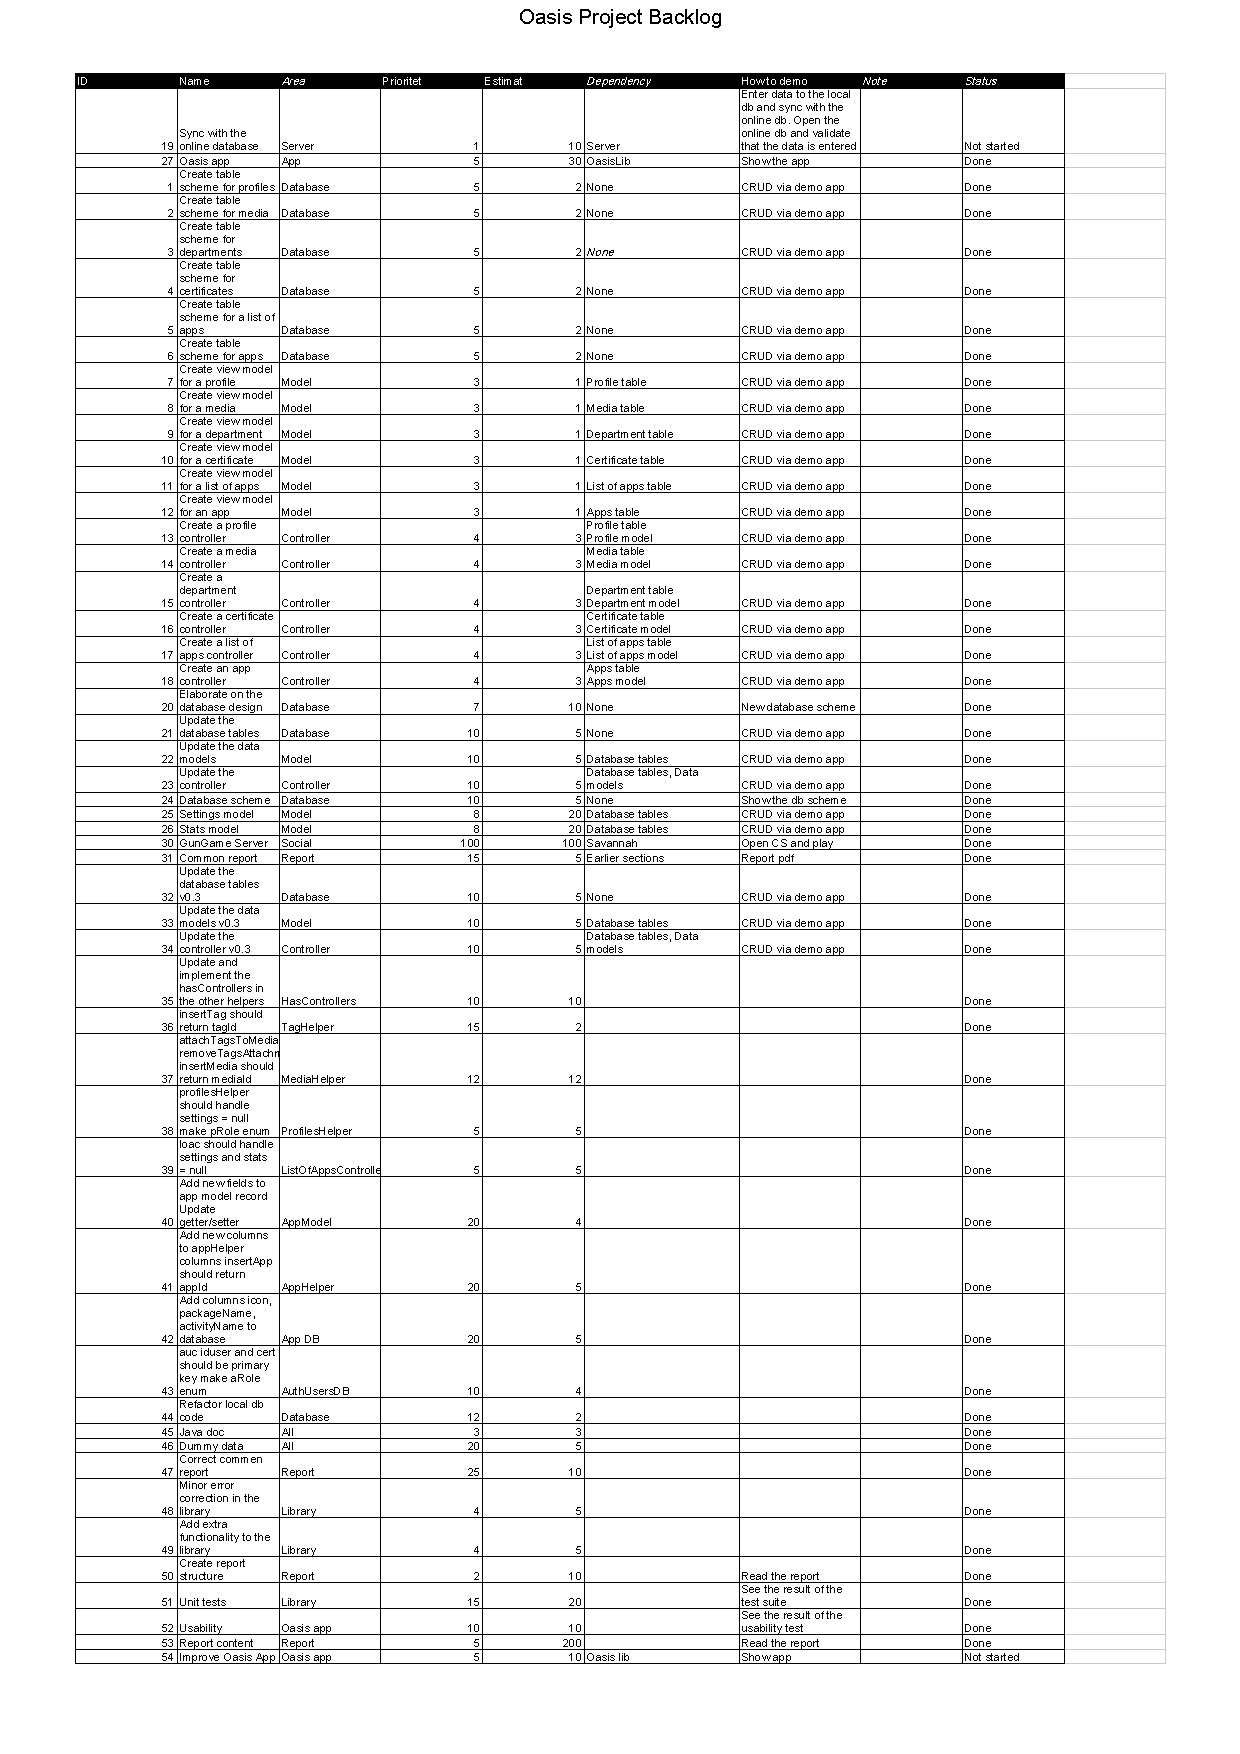
\includegraphics[width=\textwidth]{Images/OasisProjectBacklog}
	\caption{An overview of the Oasis project backlog.}
	\label{fig:projectBacklog}
\end{figure}

\chapter{Burndown Charts and Sprint Backlogs}
\label{sec:burn_back}
Here are an overview of all the sprints in this project.
	
\begin{figure}[H]
	\centering
		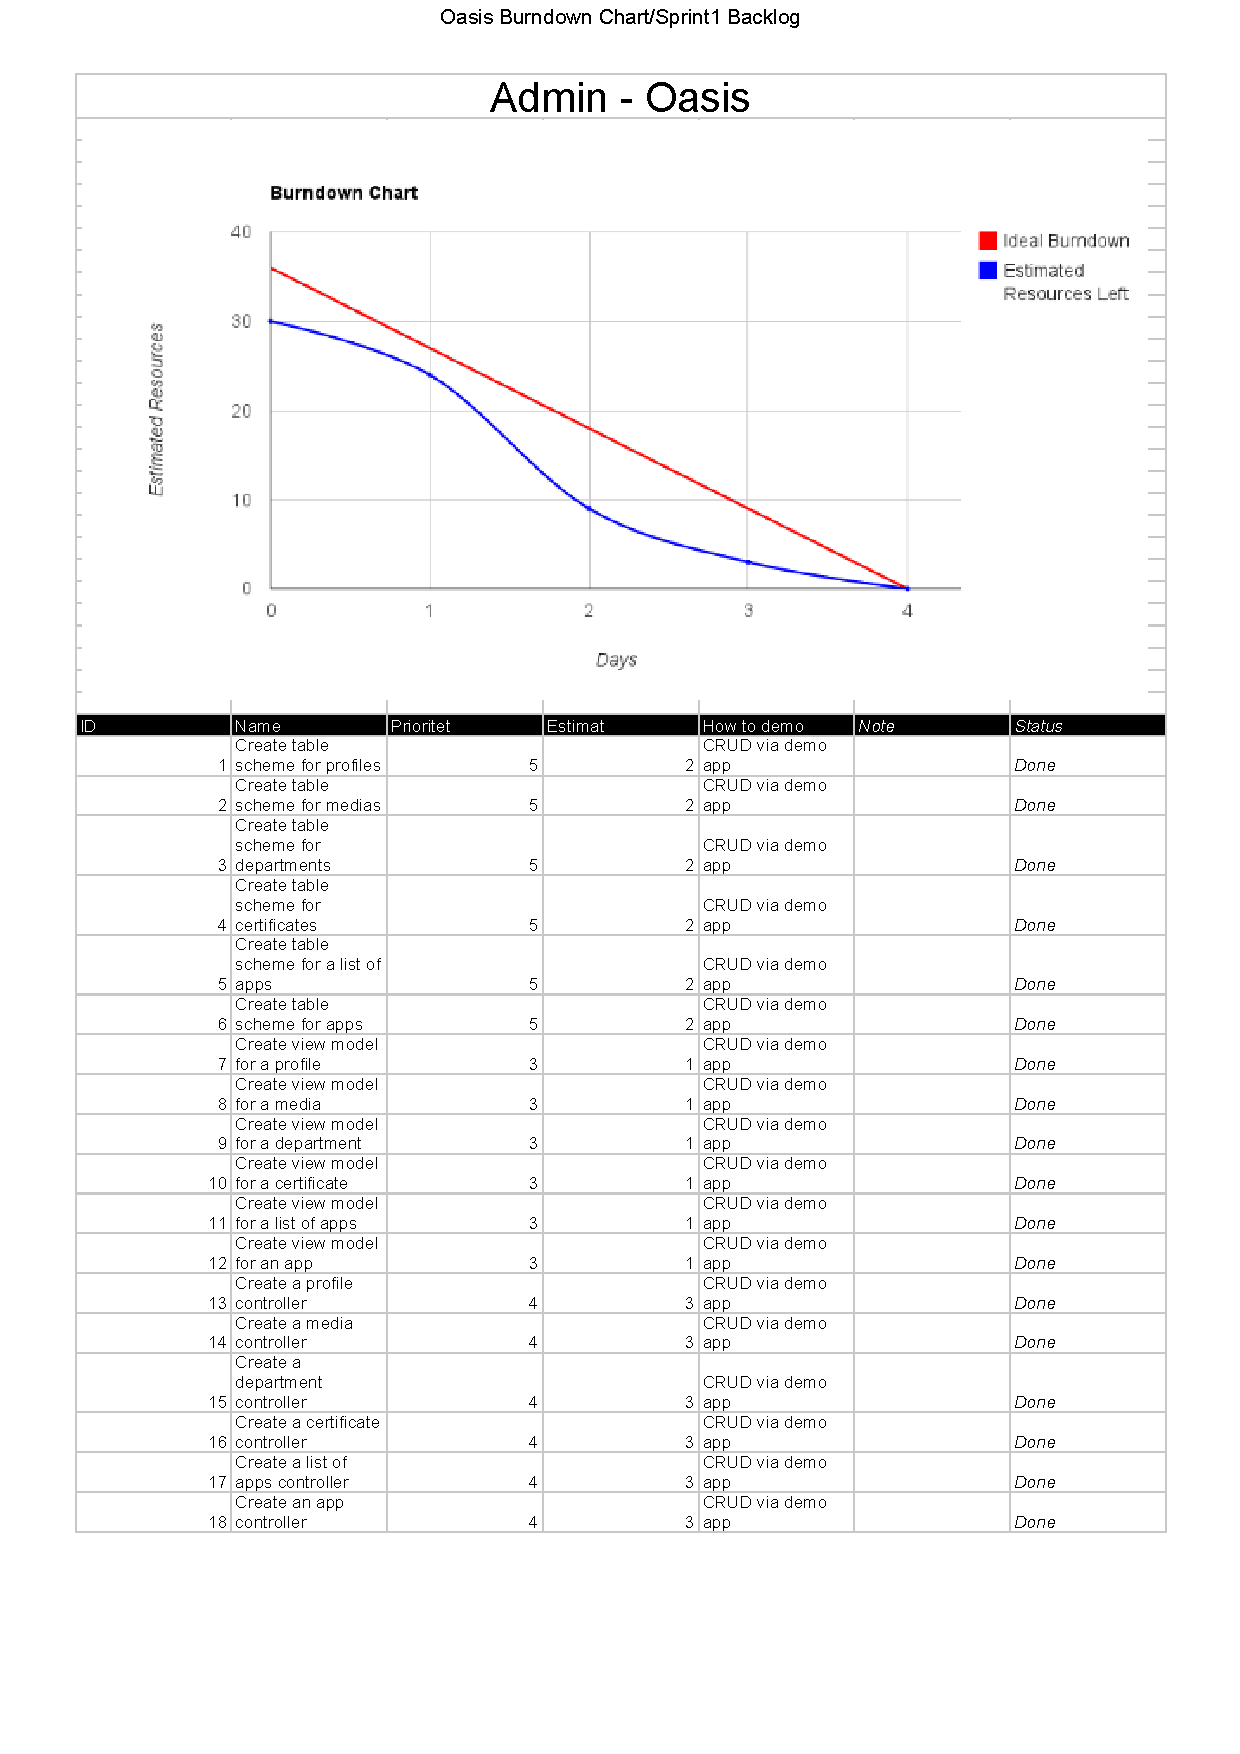
\includegraphics[width=\textwidth]{Images/sprint_backlogs/Oasis_Burndown_Chart_-_Sprint1_Backlog}
	\caption{The burndown chart and sprint backlog from sprint 1.}
	\label{fig:sprint1}
\end{figure}

\begin{figure}[H]
	\centering
		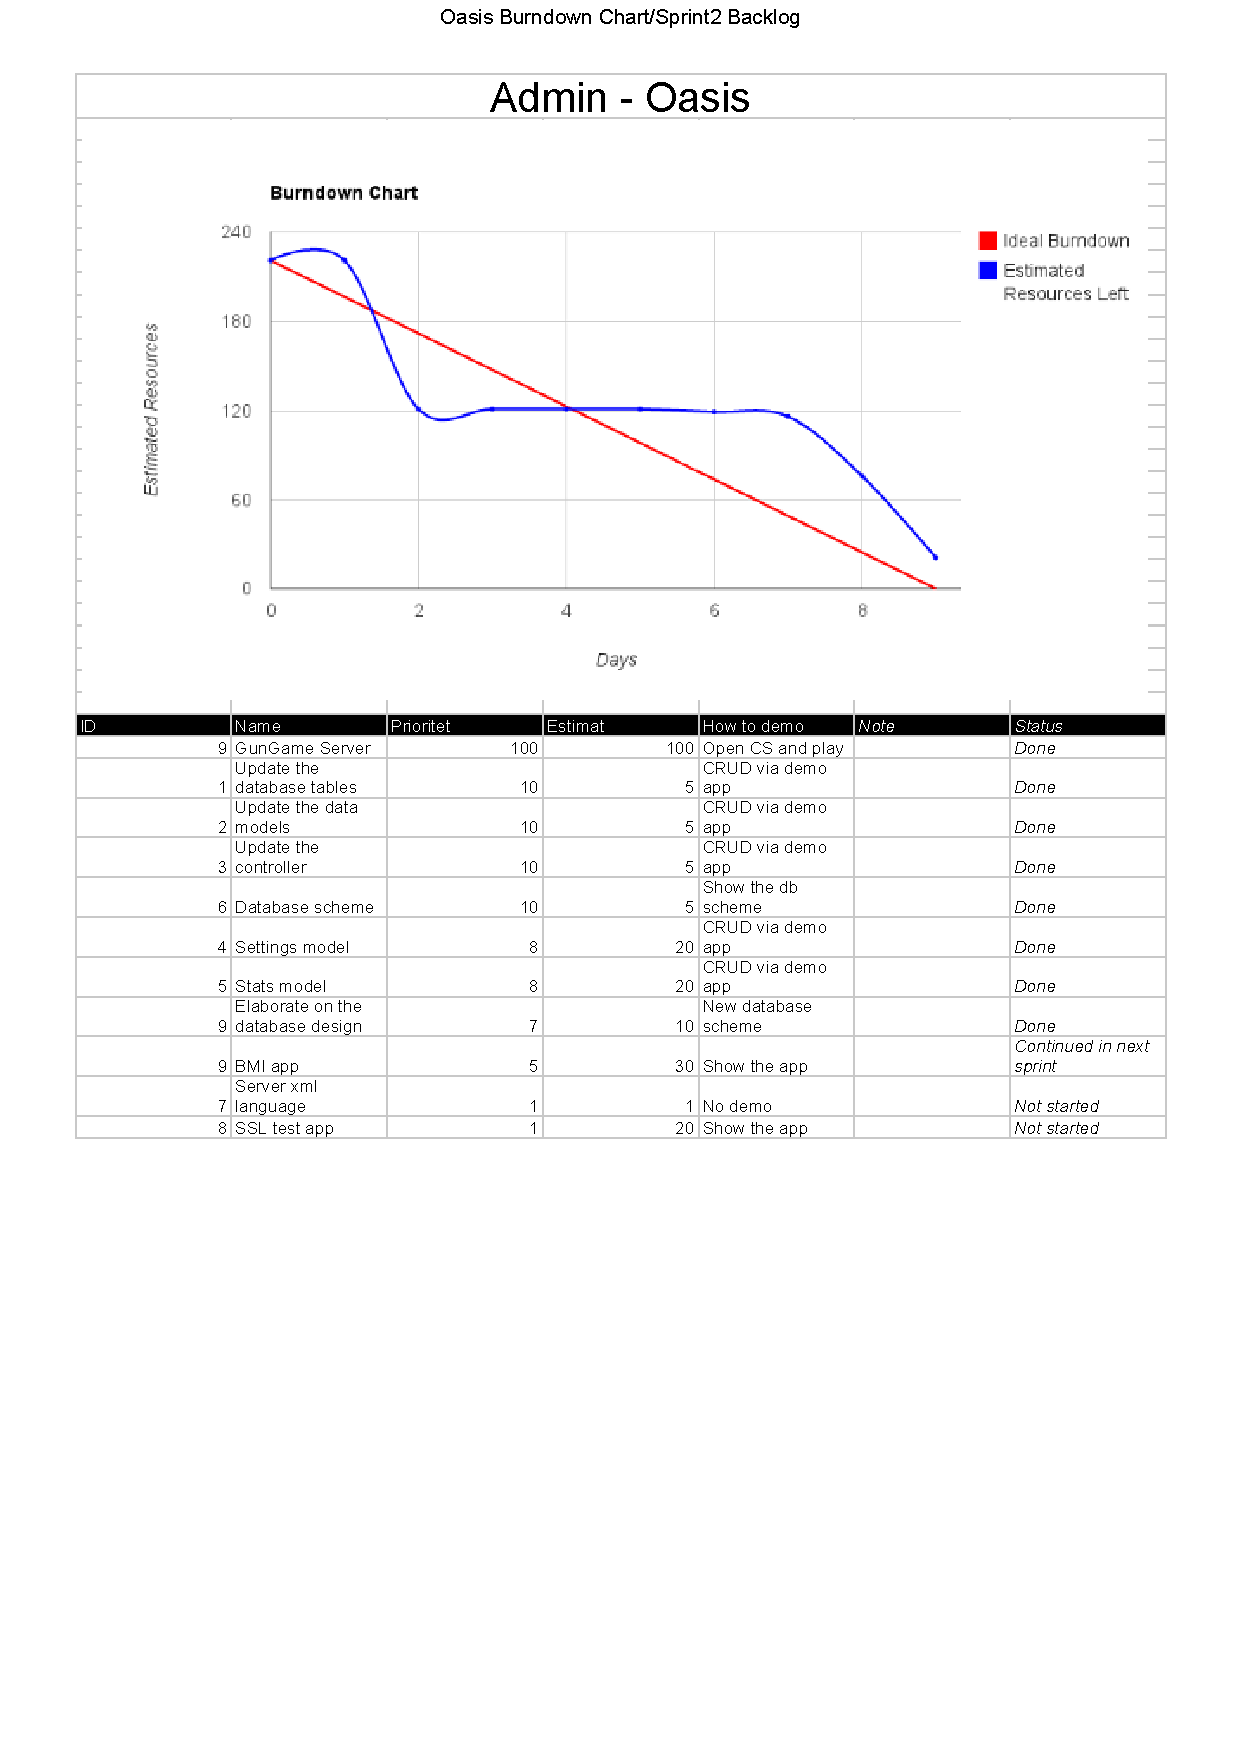
\includegraphics[width=\textwidth]{Images/sprint_backlogs/Oasis_Burndown_Chart_-_Sprint2_Backlog}
	\caption{The burndown chart and sprint backlog from sprint 2.}
	\label{fig:sprint2}
\end{figure}

\begin{figure}[H]
	\centering
		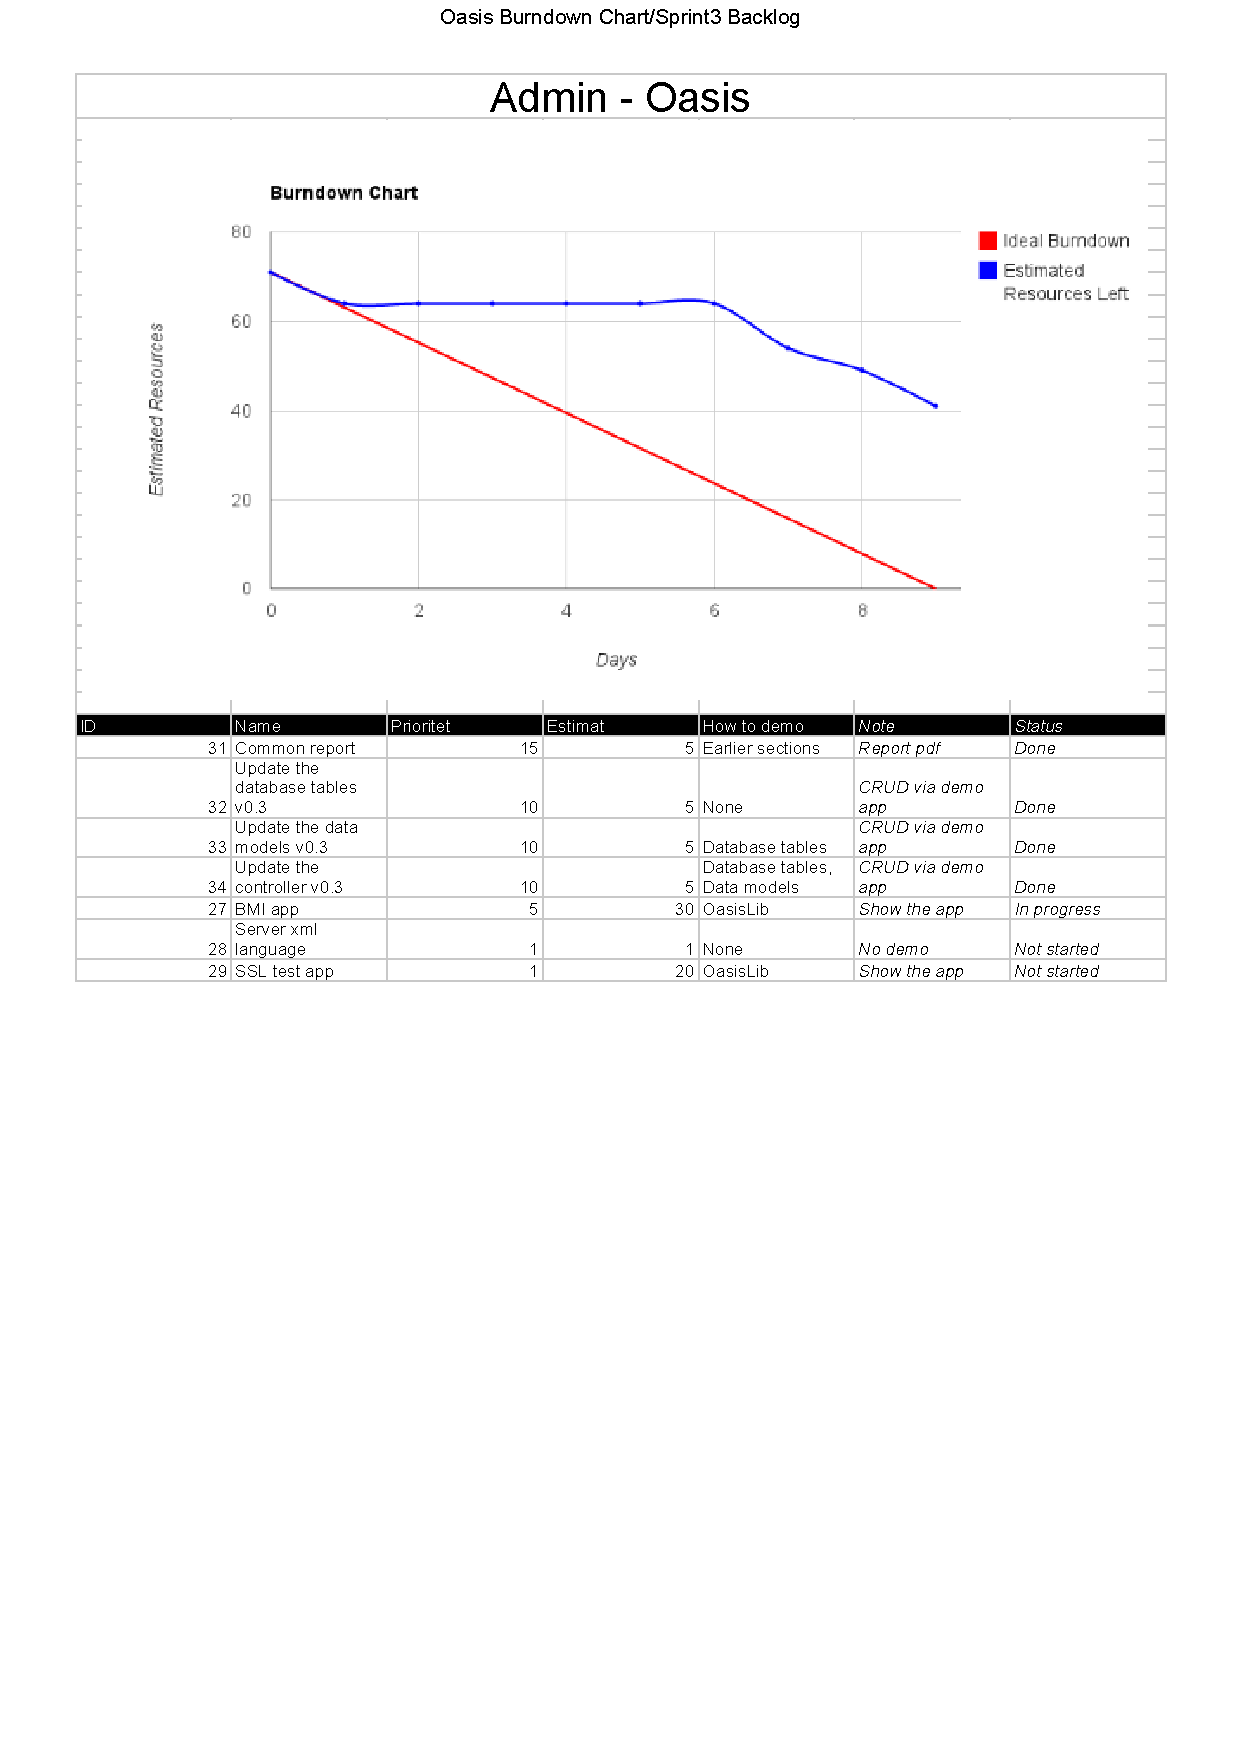
\includegraphics[width=\textwidth]{Images/sprint_backlogs/Oasis_Burndown_Chart_-_Sprint3_Backlog}
	\caption{The burndown chart and sprint backlog from sprint 3.}
	\label{fig:sprint3}
\end{figure}

\begin{figure}[H]
	\centering
		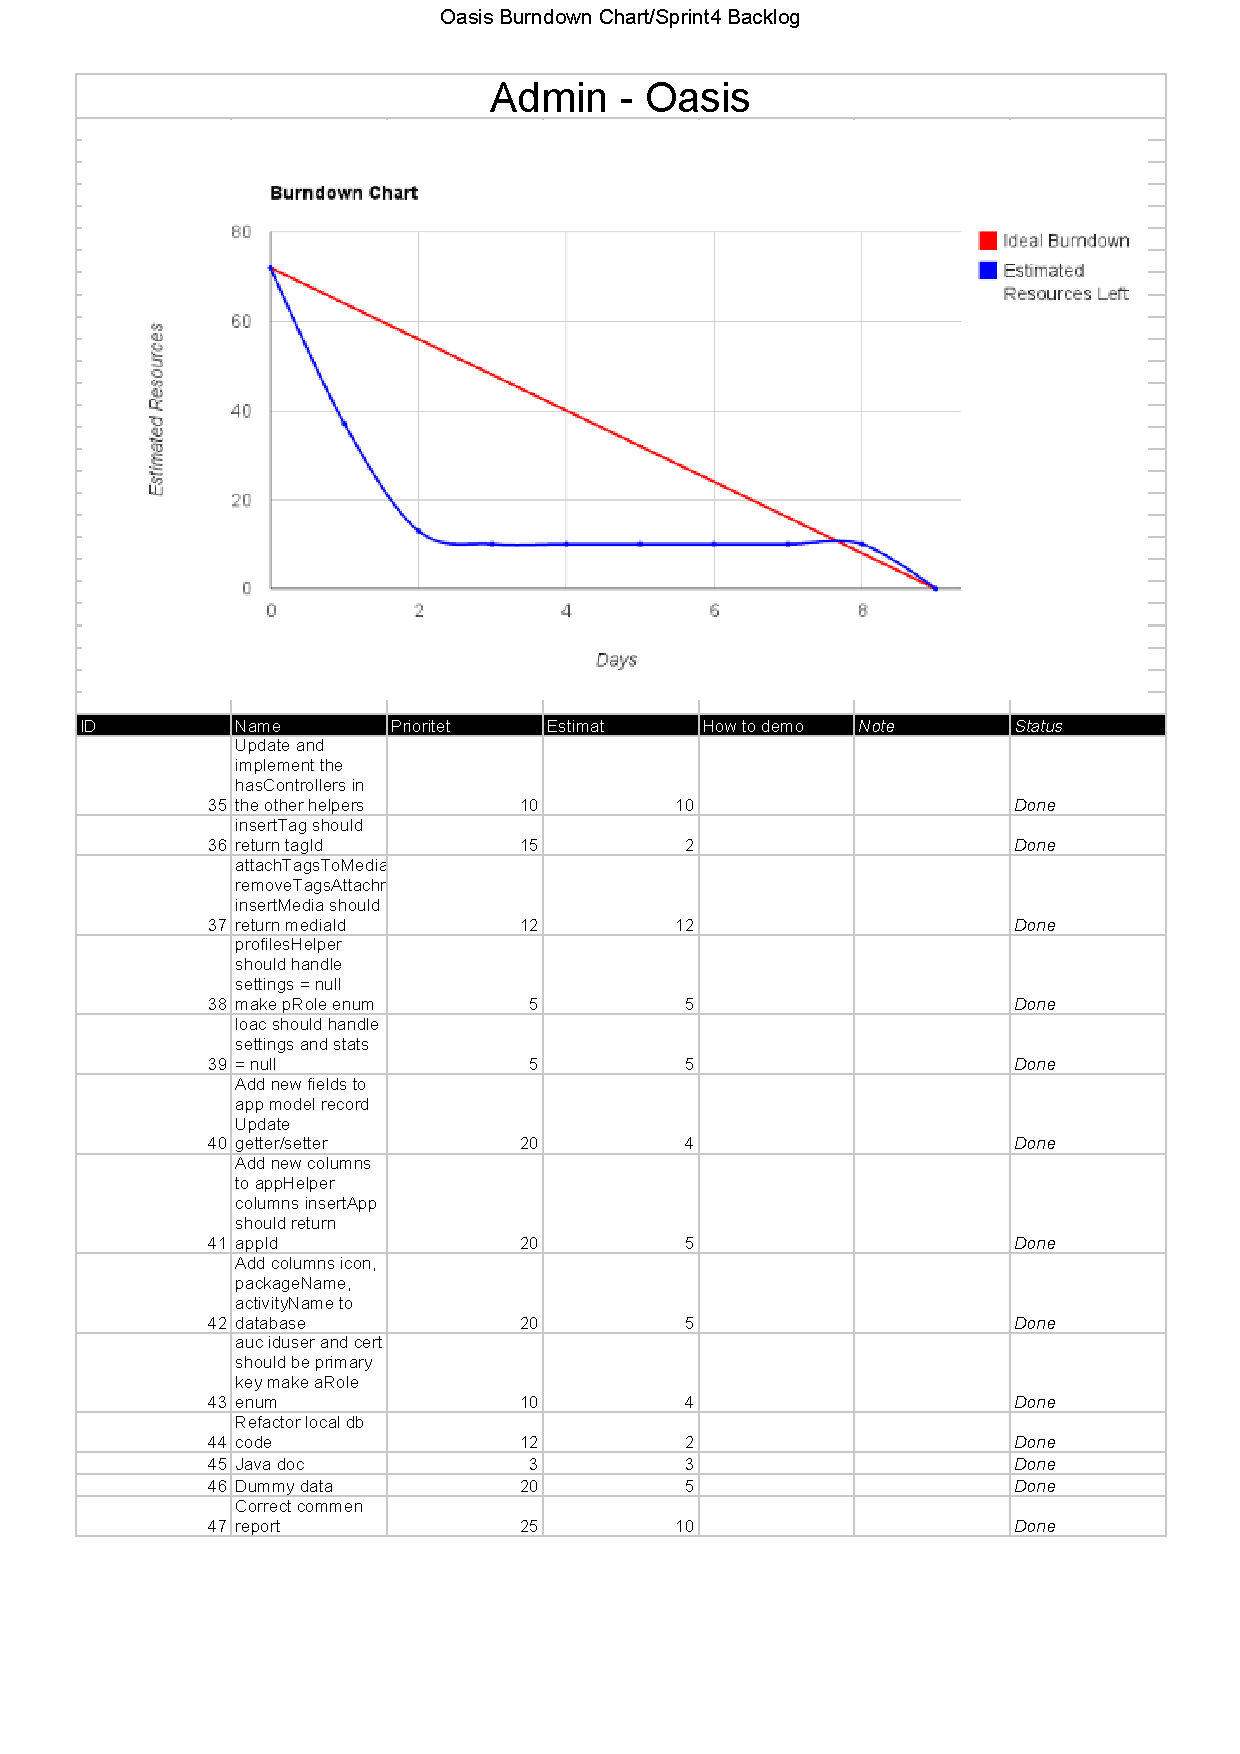
\includegraphics[width=\textwidth]{Images/sprint_backlogs/Oasis_Burndown_Chart_-_Sprint4_Backlog}
	\caption{The burndown chart and sprint backlog from sprint 4.}
	\label{fig:sprint4}
\end{figure}

\begin{figure}[H]
	\centering
		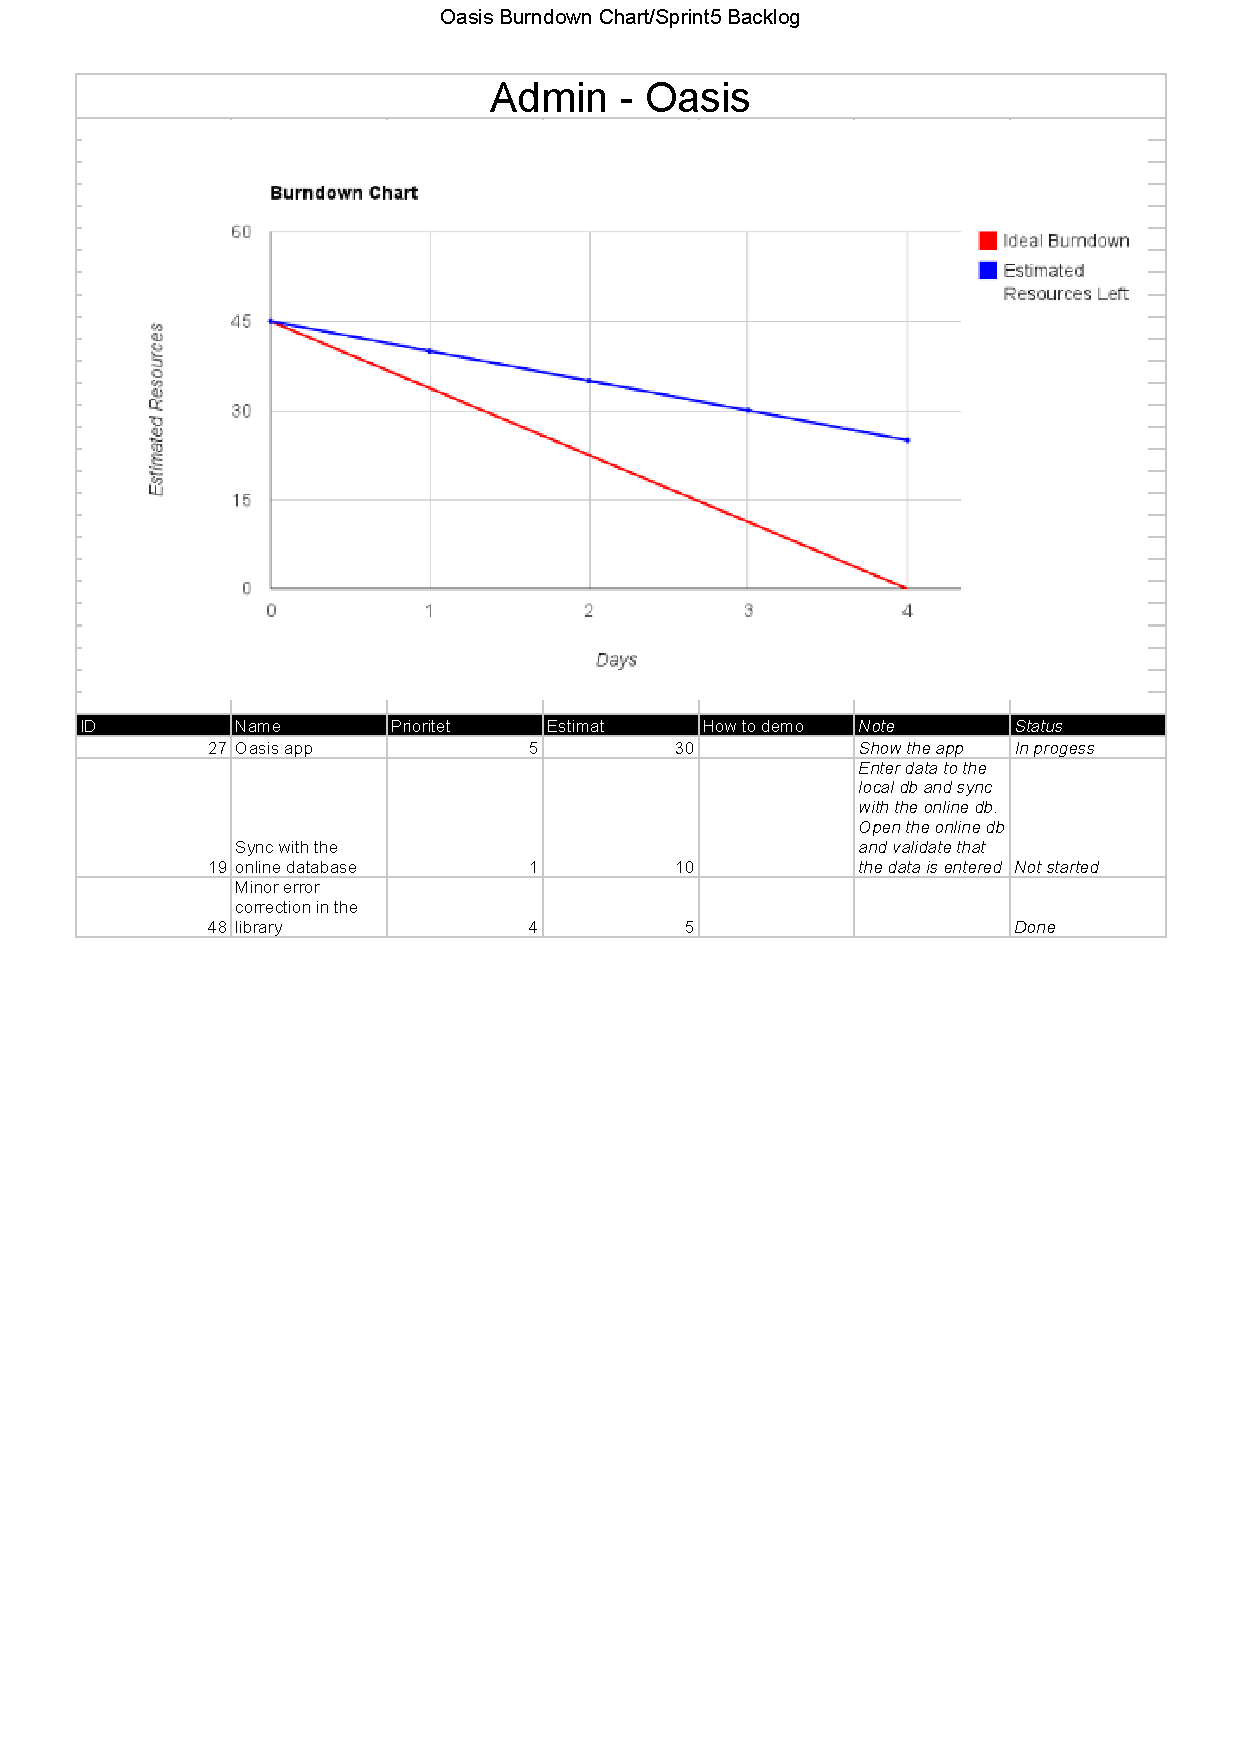
\includegraphics[width=\textwidth]{Images/sprint_backlogs/Oasis_Burndown_Chart_-_Sprint5_Backlog}
	\caption{The burndown chart and sprint backlog from sprint 5.}
	\label{fig:sprint5}
\end{figure}

\begin{figure}[H]
	\centering
		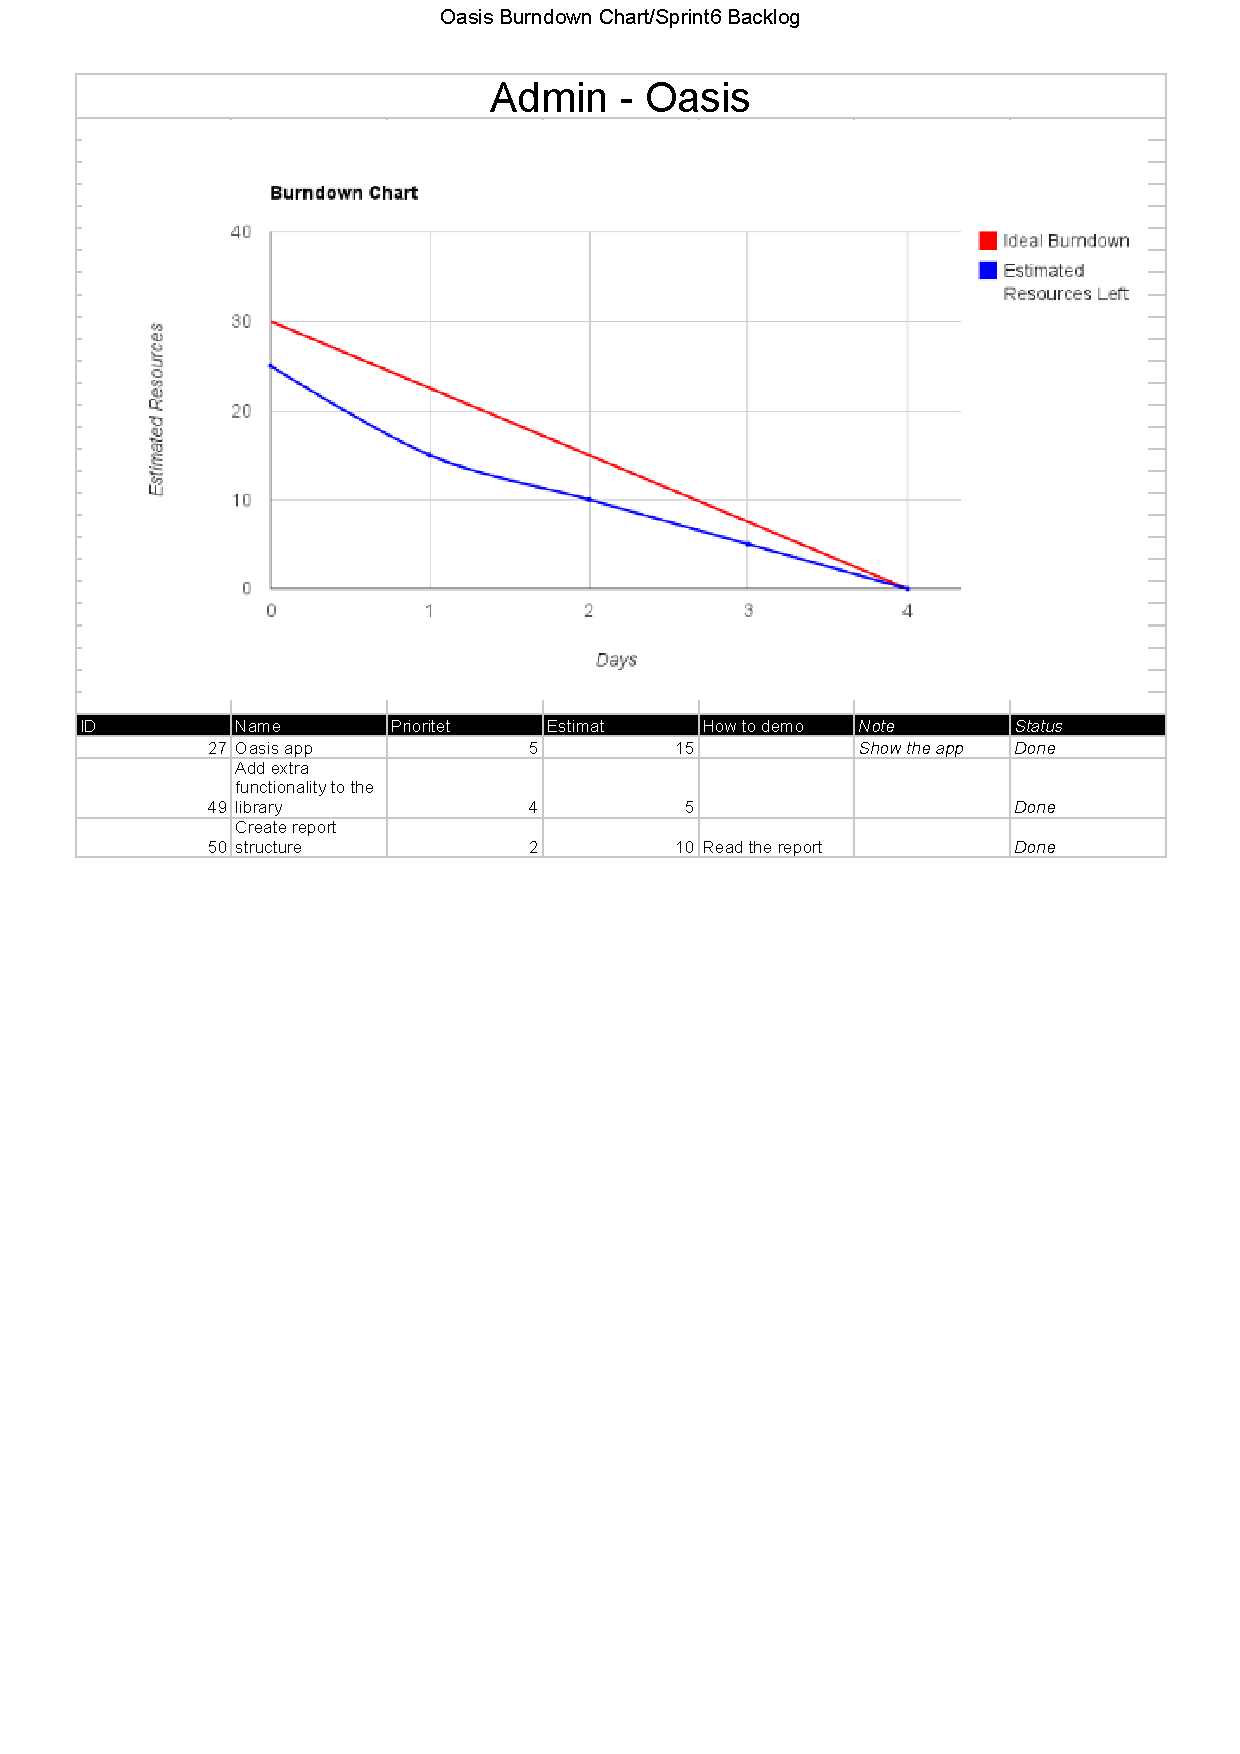
\includegraphics[width=\textwidth]{Images/sprint_backlogs/Oasis_Burndown_Chart_-_Sprint6_Backlog}
	\caption{The burndown chart and sprint backlog from sprint 6.}
	\label{fig:sprint6}
\end{figure}

\begin{figure}[H]
	\centering
		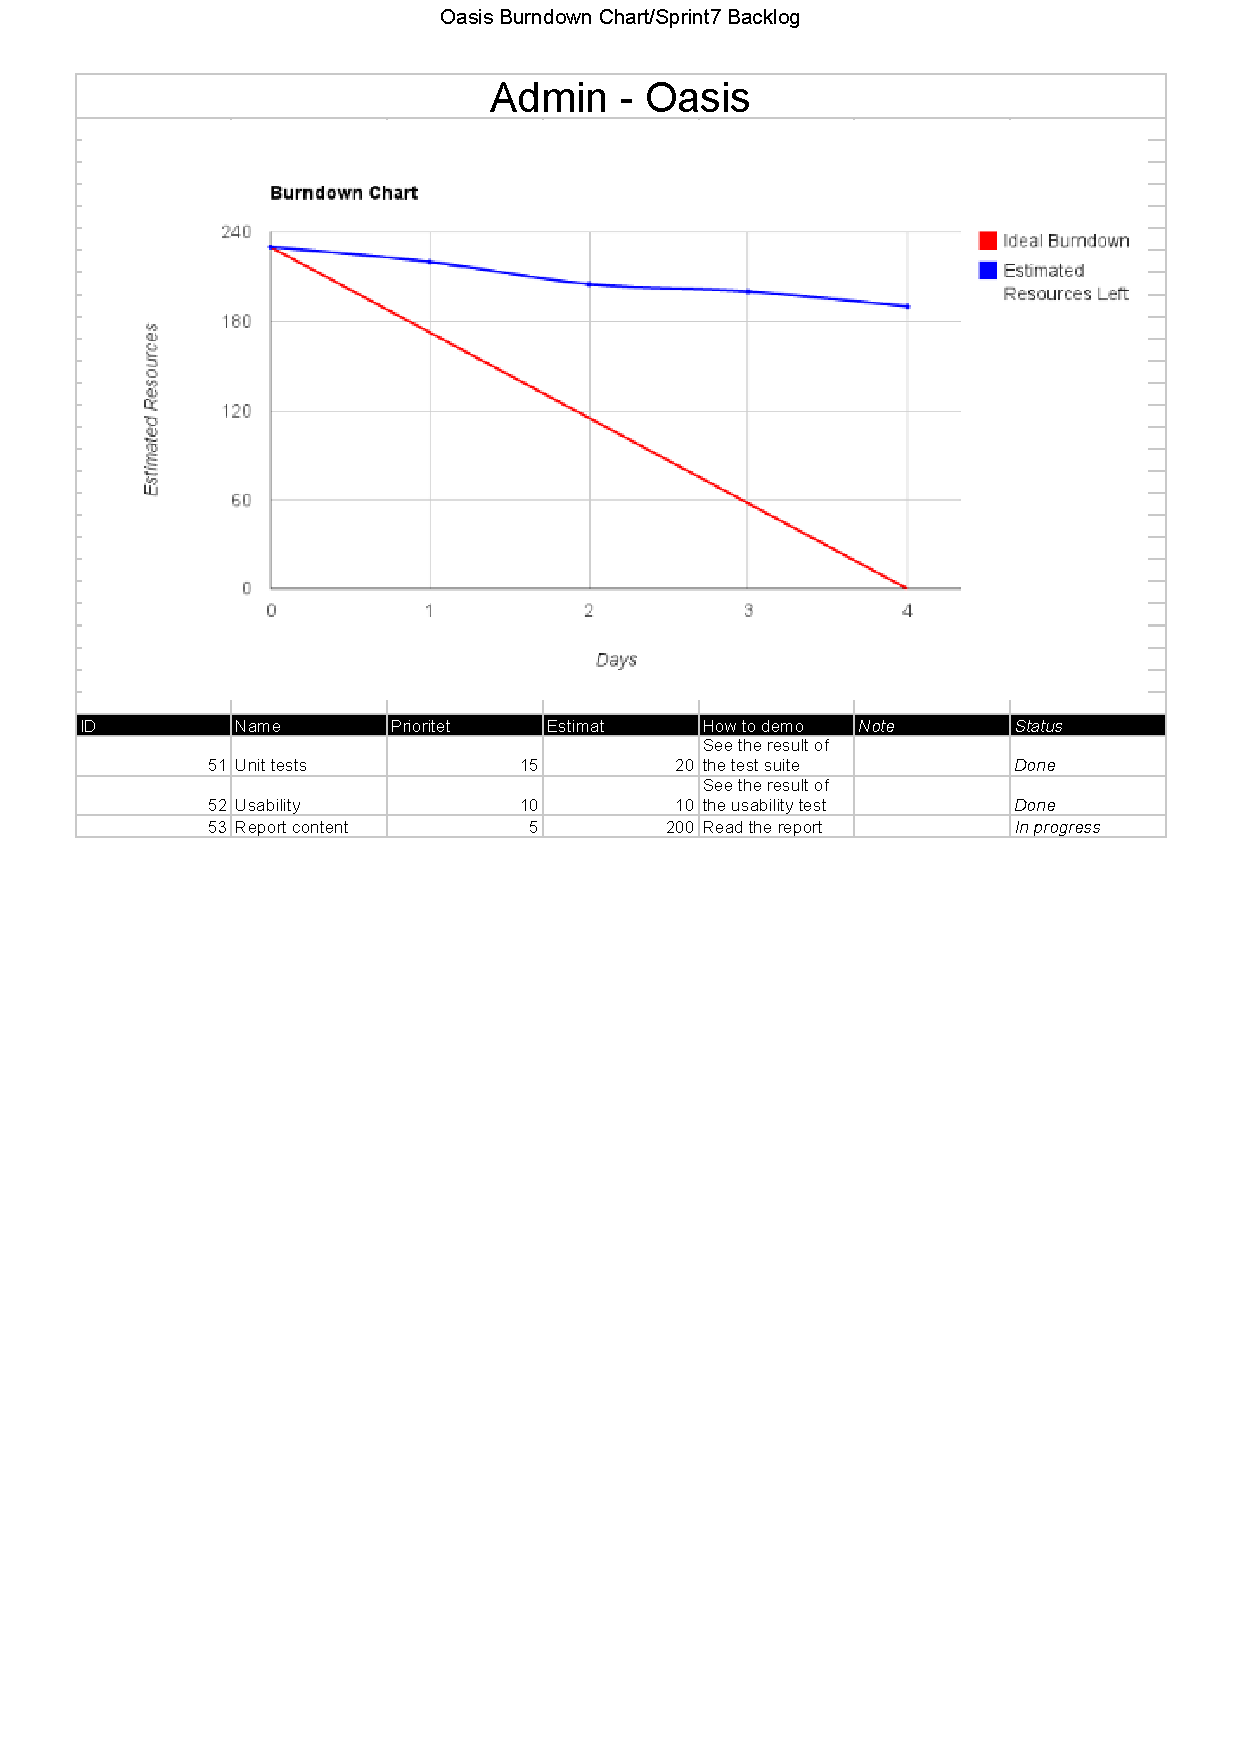
\includegraphics[width=\textwidth]{Images/sprint_backlogs/Oasis_Burndown_Chart_-_Sprint7_Backlog}
	\caption{The burndown chart and sprint backlog from sprint 7.}
	\label{fig:sprint7}
\end{figure}

\begin{figure}[H]
	\centering
		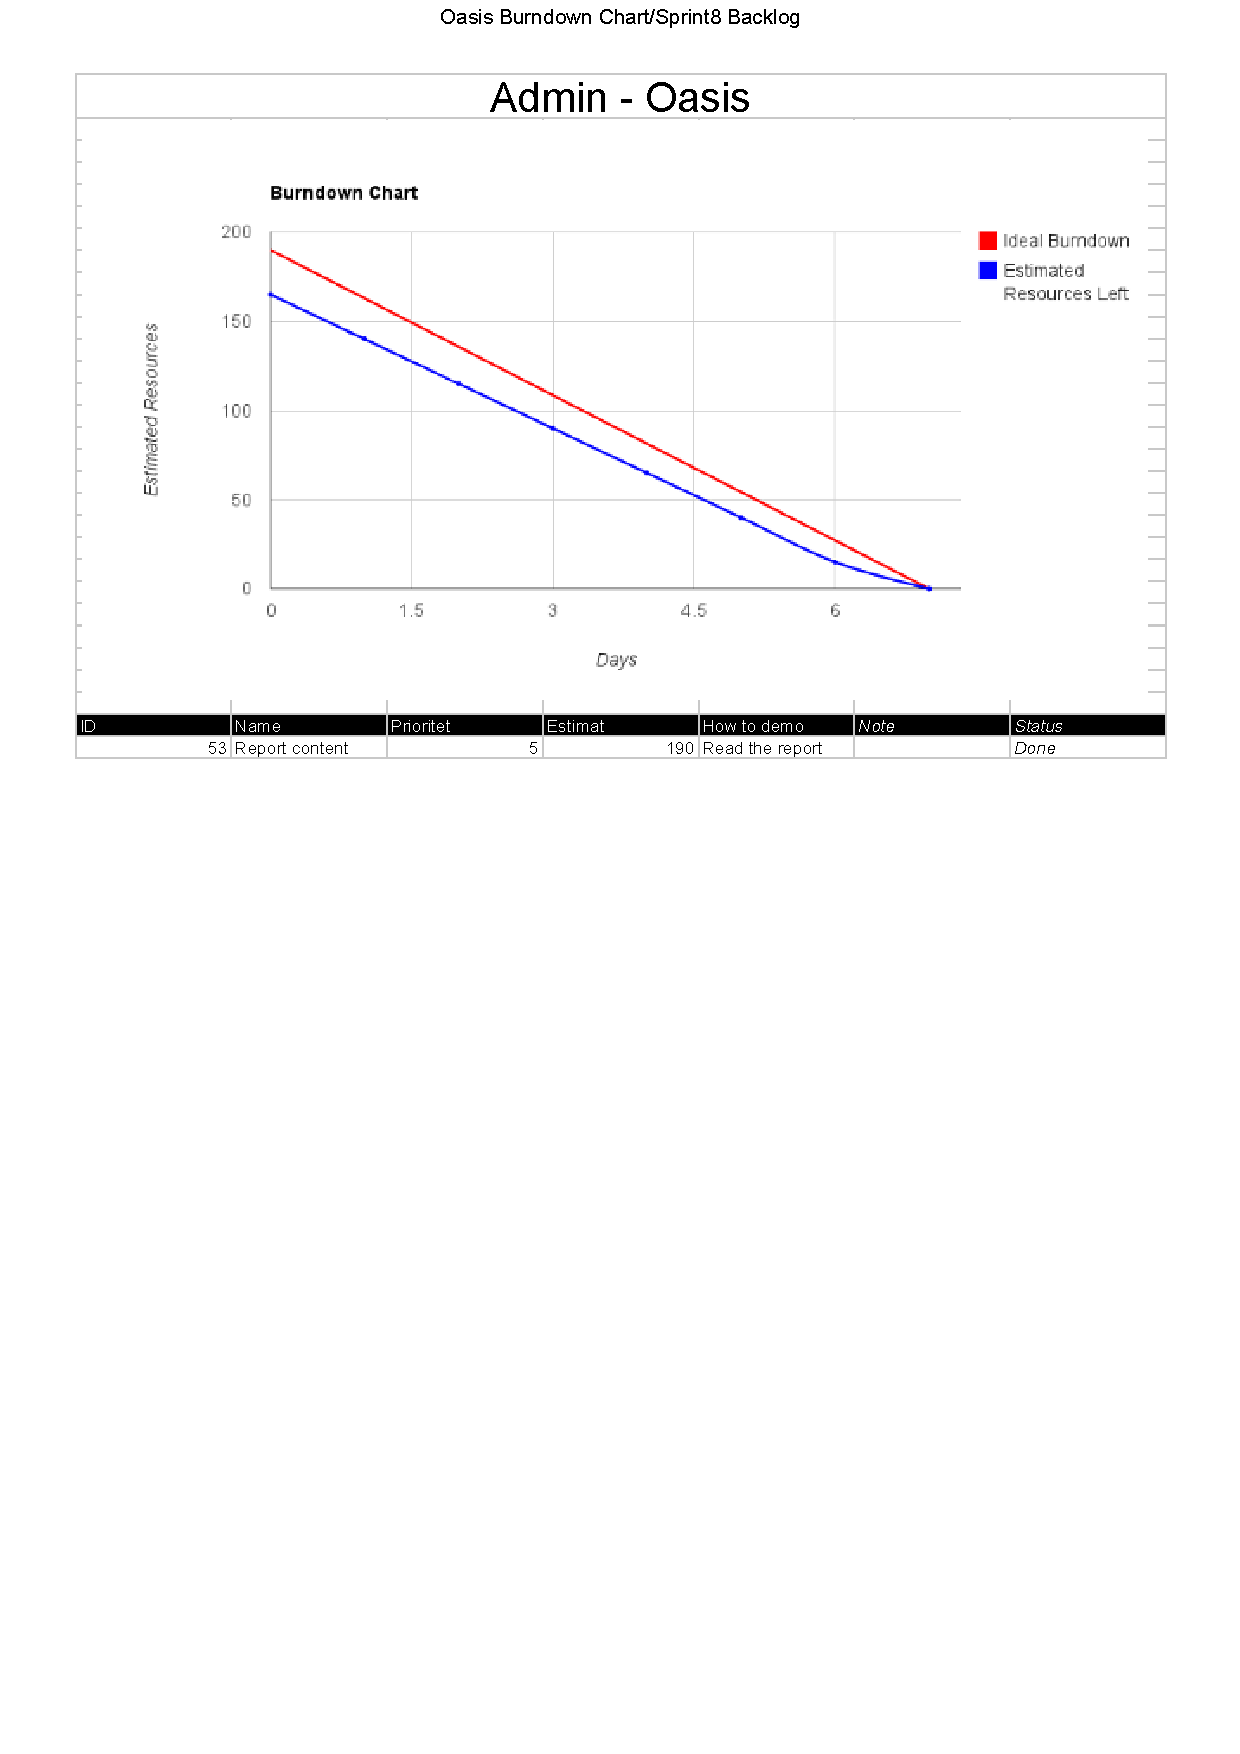
\includegraphics[width=\textwidth]{Images/sprint_backlogs/Oasis_Burndown_Chart_-_Sprint8_Backlog}
	\caption{The burndown chart and sprint backlog from sprint 8.}
	\label{fig:sprint8}
\end{figure}

\chapter{Change Log}
\label{sec:change_log}
Here is the full change log for the Oasis Library -- along with the models used in it -- and the Oasis Local Database.

\begin{figure}[H]
	\centering
		\includegraphics[width=\textwidth]{Images/OasisChangeLog}
	\caption{The change log for the library and database.}
	\label{fig:change_log}
\end{figure}

\begin{figure}[H]
	\begin{center}
	
\includegraphics[width=\textwidth]{Appendix/invitation_to_usability_test.pdf}
	\end{center}
\caption{Invitation sent to the test persons of the usability test.}
\label{fig:usability_test_invitation}
\end{figure}

\chapter{Mail correspondence with Customer}
\label{sec:customerReq}
\subsection{Mail To Customer}
Hej Kristine

Vi er blevet tildelt dig som kontakt person i forbindelse med vores projekt. Som n\ae{}vnt sidst s\aa{} arbejder vi p\aa{} at udvikle applikationer til android, som kan bruges enten af jer som p\ae{}dagoger og m\aa{}ske af autisterne p\aa{} sigt. Vi vil udvikle flere forskellige applikationer, og vi vil gerne l\o{}bende aftale m\o{}der med dig, hvor vi kan vise det samlede produkt som er lavet. P\aa{} den m\aa{}de kan vi f\aa{} feedback p\aa{} hvad der g\aa{}r godt og hvad der er knap s\aa{} godt.

Vores udviklings gruppe best\aa{}r af tre personer og vi skal lave en applikation der kan hj\ae{}lpe med at lave profiler der passer til b\o{}rnene. 

Da vi stadig kun er i gang med at planl\ae{}gge mener vi ikke at det er n\o{}dvendigt at holde et m\o{}de endnu. Men vi har nogen sp\o{}rgsm\aa{}l som vi gerne vil have dig til at svare p\aa{}:

\subsubsection{Hvilke informationer gemmer i omkring det enkelte barn?}
\begin{itemize}
	\item Journal nummer?
	\item Person nummer?
	\item Navn?
	\item Alder?
	\item S\ae{}rlige behov?
\end{itemize}

\subsubsection{a - Ur}
a1. Vil barnet kunne forst\aa{} at en hel cirkel kan have forskelligt tidsinterval?
a1.1 Eller er det bedst hvis cirklen har et fast tidsrum fx 1 time?
\\
a2. Hvis man skal m\aa{}le et tidsinterval p\aa{} uret, er det s\aa{} bedst at lade uret efterligne et almindeligt ur med 12 timer eller et stop-ur med kun 1 time?

\subsubsection{b - Timeglas}
b1. Vil barnet kunne forst\aa{} at det samme timeglas med den samme m\ae{}ngde sand kan varierer i tid?
\\
b2. Er det bedst at man varierer i m\ae{}ngden af sand i timeglasset eller at man varierer i timeglassets st\o{}rrelse?

\subsubsection{c - Aktivitetstid}
c1. Vil barnet kunne forst\aa{} at en linje der g\aa{}r hele vejen hen over sk\ae{}rmen kan varierer i tidsinterval?      
c1.1 Eller er det bedre hvis linjen har et fast tidsinterval og fx en halv linje derfor svarer til en halv time og en hel linje til en hel time? 

\subsubsection{d - Dagsplan}
d1. Hvis man laver en visuel dagsplan er det s\aa{} bedst at man laver et interval som viser tiden imellem to aktiviteter, eller at man viser alle aktiviter i l\o{}bet af dagen kombineret med en tidslinje?

\subsection{Mail From Customer}
Hej.
Tak for jeres mail.
Jeg skal besvare jeres mail s\aa{} godt som muligt, og s\aa{} m\aa{} i give lys hvis i har brug for at jeg uddyber.
\\
Vedr. informationer vedr. barnet:
Vi benytter et elektronisksystem som hedder, EKJ, hvor alle oplysninger p\aa{} b\o{}rnene er gemt. Det vil sige, pers. nr., adresse oplysninger, indbydelser, handleplaner og referater fra diverse m\o{}der.
 \\
UR: Hvis det er tydeligt vist at ``tiden g\aa{}r'' /skiven bliver mindre/forsvinder, som tiden g\aa{}r, vil barnet forst\aa{} meningen med uret. For at indikere forskellig tid, kan man benytte forskellige farvet baggrunde. Lilla:5 min. Gr\o{}n:10 min osv. Vi benytter kun kortere tidsintervaller,(1. min. 3. min. 5 min. -op til ca. 10-15. min) da 1 time er for abstrakt.
\\
Timeglas: Hvis der er en tydelig markering af tidsintervallet, som beskrevet ovenfor, er det muligt at bruge samme timeglas. Tror det vil give bedst forst\aa{}else for barnet, hvis m\ae{}ngden af sand varieres efter tid. 
\\
Aktivitetstid og dagsplan: (Tror J) Aktivitetstid kan bruges ved, at tiden bliver indikeret af m\ae{}ngden af aktiviteter.
 - Alts\aa{} 3-5 viste aktiviteter af gangen, og ikke s\aa{} meget om det er en time eller 15 min. 
Tiden kunne v\ae{}re en mulighed at tilf\o{}re, om n\o{}dvendigt. Mange af vores b\o{}rn har manglende fornemmelse for tid, og ofte har de brug for at se sm\aa{} konkrete sekvenser/beskeder frem for mange over l\ae{}ngere tid.
Derfor vil jeg tror de bedst kan overskue \textonehalf{} dag af gangen, men stadig have mulighed for at have dagen p\aa{} skemaet, hvor det kan vises i sekvenser.
\\
Jeg har samlet de to ovenst\aa{}ende punkter, da de nemt kommer til at gribe ind i hinanden.
Vores ugeskemaer i b\o{}rnehaven er vist med internationale farver, dem vil i ligeledes kunne benytte til at tydeligg\o{}re ugedagene.
Mandag: Gr\o{}n, Tirs.: Lilla, Ons.: orange, tors.: bl\aa{}, Fre.: gul, l\o{}r.: r\o{}d og s\o{}ndag: hvid.
\\
H\aa{}ber dette er uddybende nok, ellers m\aa{} i gerne skrive eller ringe til mig hvis det er nemmere.
\\
Ser  frem til at h\o{}rer fra jer igen.
\section{Notes from Interview}
\label{InterviewMette}
\textit{This is notes from an interview with Mette Als Andreasen, an educator at Birken in Langholt, Denmark.}

N�r tiden l�ber ud (kristian har tage et billede):\\
F�rdig - symbol\\
G� til skema - symbol\\
Taget fra boardmaker\\

Kunne v�re godt hvis man kunne s�tte egne billeder ind som start/stop symboler.\\


R�d farve $=$ nej, stop, aflyst.\\

De har s�dan et ur p� 60 minutter hvor tid tilbage er markeret med r�d, og s� bipper den lige kort n�r den er f�rdig.\\
  Det ville v�re fint hvis de kunne bruge sort/hvid til dem der ikke kan h�ndtere farver, men ogs� kan v�lge farver.\\

Stop-ur:\\
en fast timer p� 60 minutter $+$ en customizable som ikke ser helt magen til ud, som f.eks, kan v�re p� 5, 10 eller 15 minutter for en hel cirkel.\\

timeglas:\\
skift farve p� timeglassene, men ikke n�dvendigvis g�re dem st�rre. Kombinere med mere/mindre sand. Eventuelt kombinere med et lille digitalt ur, til dem der har brug for det, skal kunne sl�es til og fra.\\

Dags-plan:\\
ikke s�rlig relevant til de helt sm� og ikke s�rligt velfungerende b�rn. Men kunne v�re rigtig godt til de lidt �ldre.\\
   En plan g�r oppefra og ned, og hvis der s� skal specificeres noget ud til aktiviteterne, s� er det fra venstre mod h�jre ud fra det nedadg�ende skema.\\

Til parrot:\\
Godt med rigtige billeder af tingene, som p�dagogerne selv kan tage, eventuelt ogs� af aktiviteter, s� pedagogerne kan have billeder af aktiviter som de kan liste efter skeamet.\\

Der var mange skemaer rundt omkring, og der henviser det sidste billede i r�kken til n�ste skema, som h�nger f.eks. p� badev�relset eller i garderoben.

\chapter{Usability Documents}
\label{app:usability_documents}

\begin{figure}[H]
	\begin{center}
	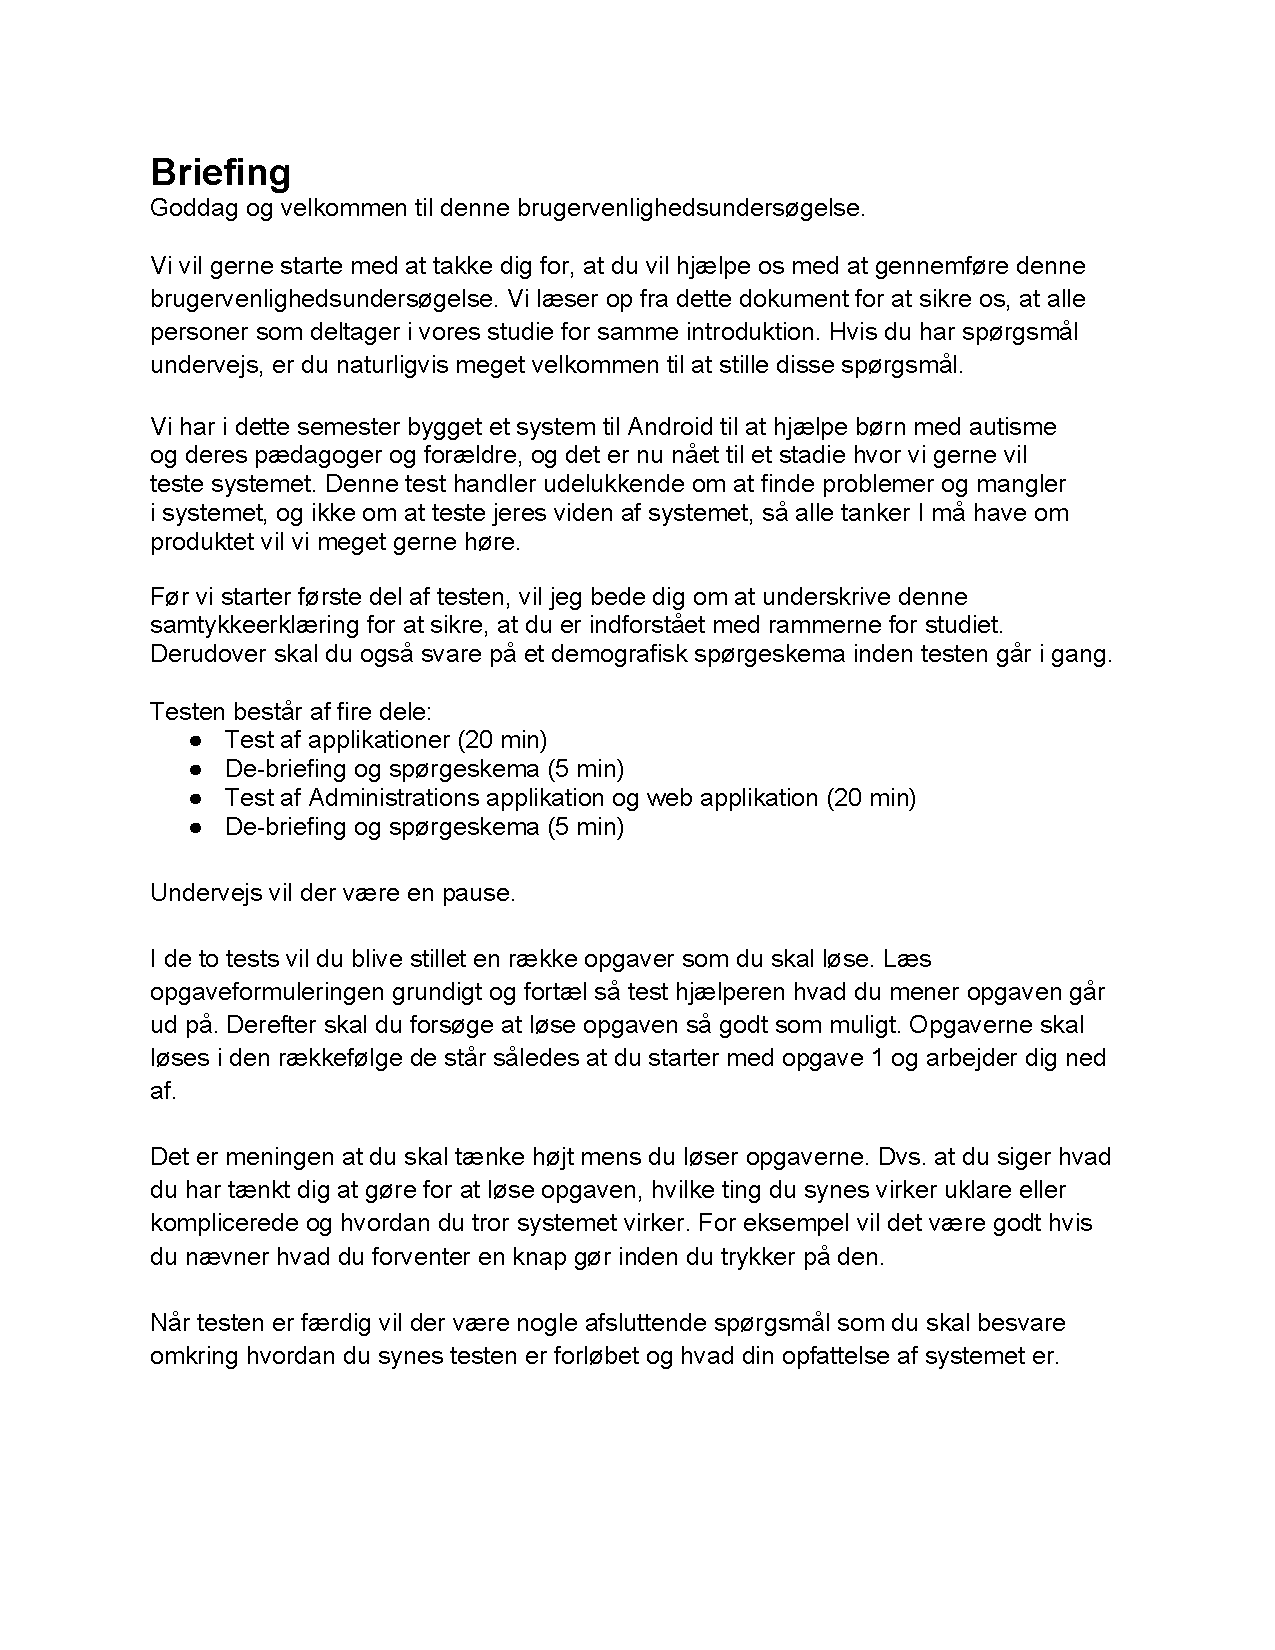
\includegraphics[width=\textwidth]{Appendix/Briefingogde-briefing}
	\end{center}
\caption{The document used to brief and de-brief the test persons.}
\label{fig:brief_debrief}
\end{figure}

\subsection{Questionnaires from usability}

\label{questionnaires}

\begin{figure}[h]
	\centering
		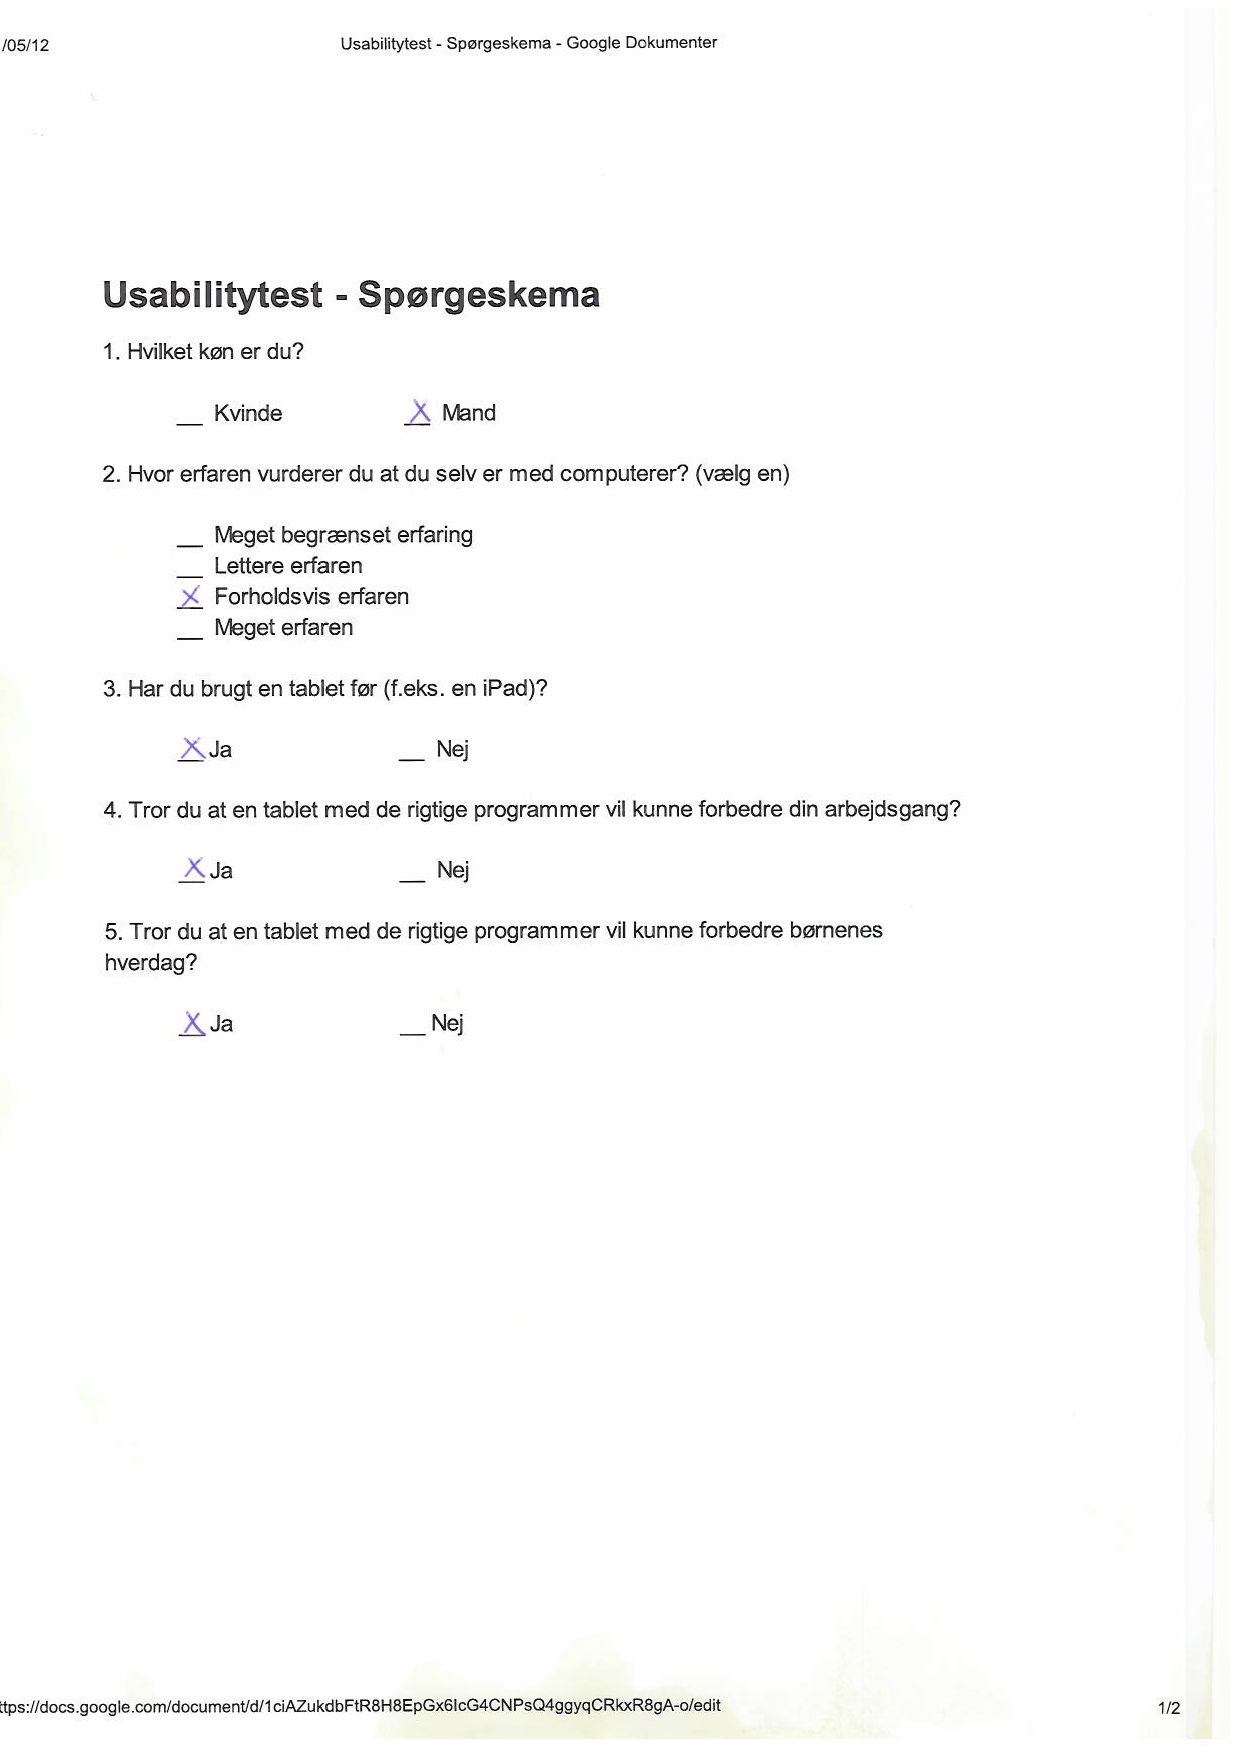
\includegraphics{Appendix/demo_d1.pdf}
	\label{fig:demo_t}
\end{figure}

\begin{figure}[h]
	\centering
		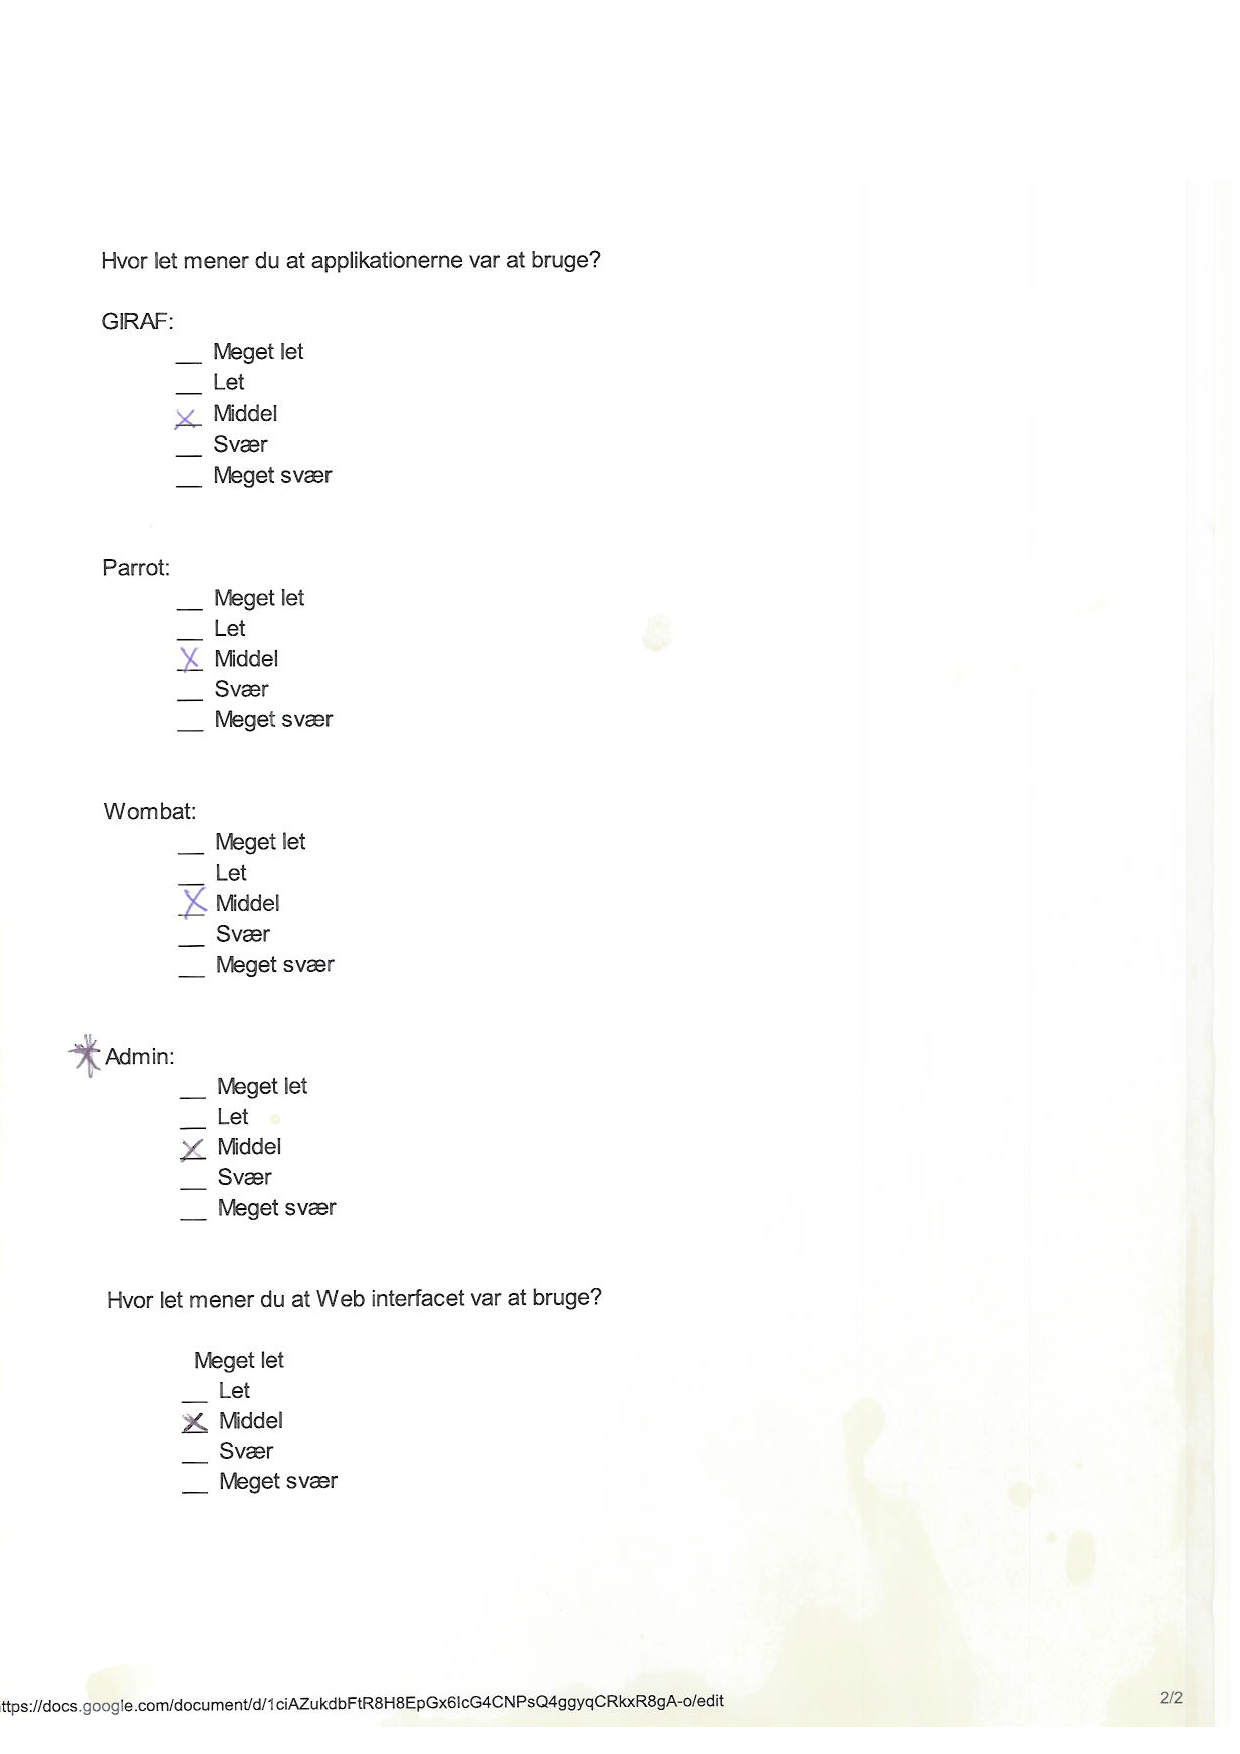
\includegraphics{Appendix/demo_d2.pdf}
	\label{fig:demo_t}
\end{figure}

\begin{figure}[h]
	\centering
		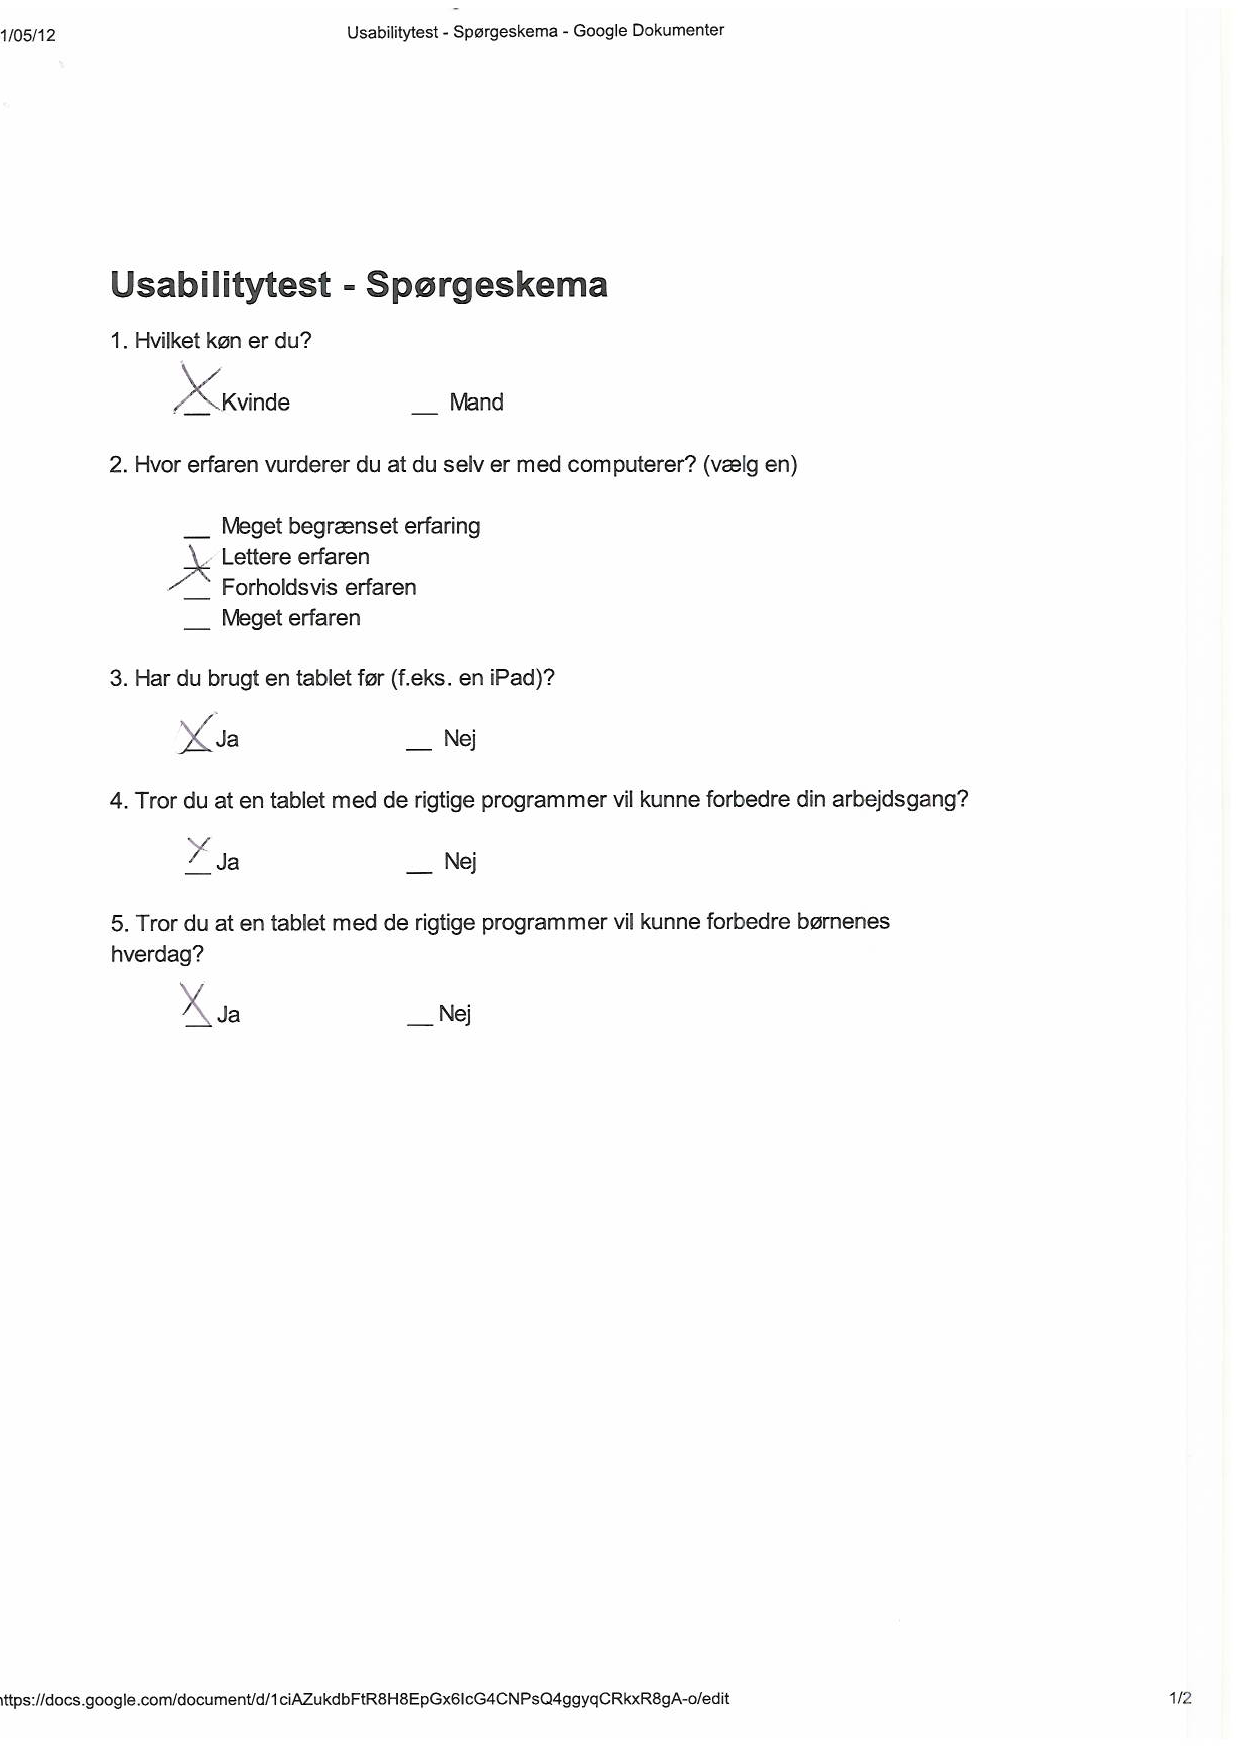
\includegraphics{Appendix/demo_m1.pdf}
	\label{fig:demo_t}
\end{figure}

\begin{figure}[h]
	\centering
		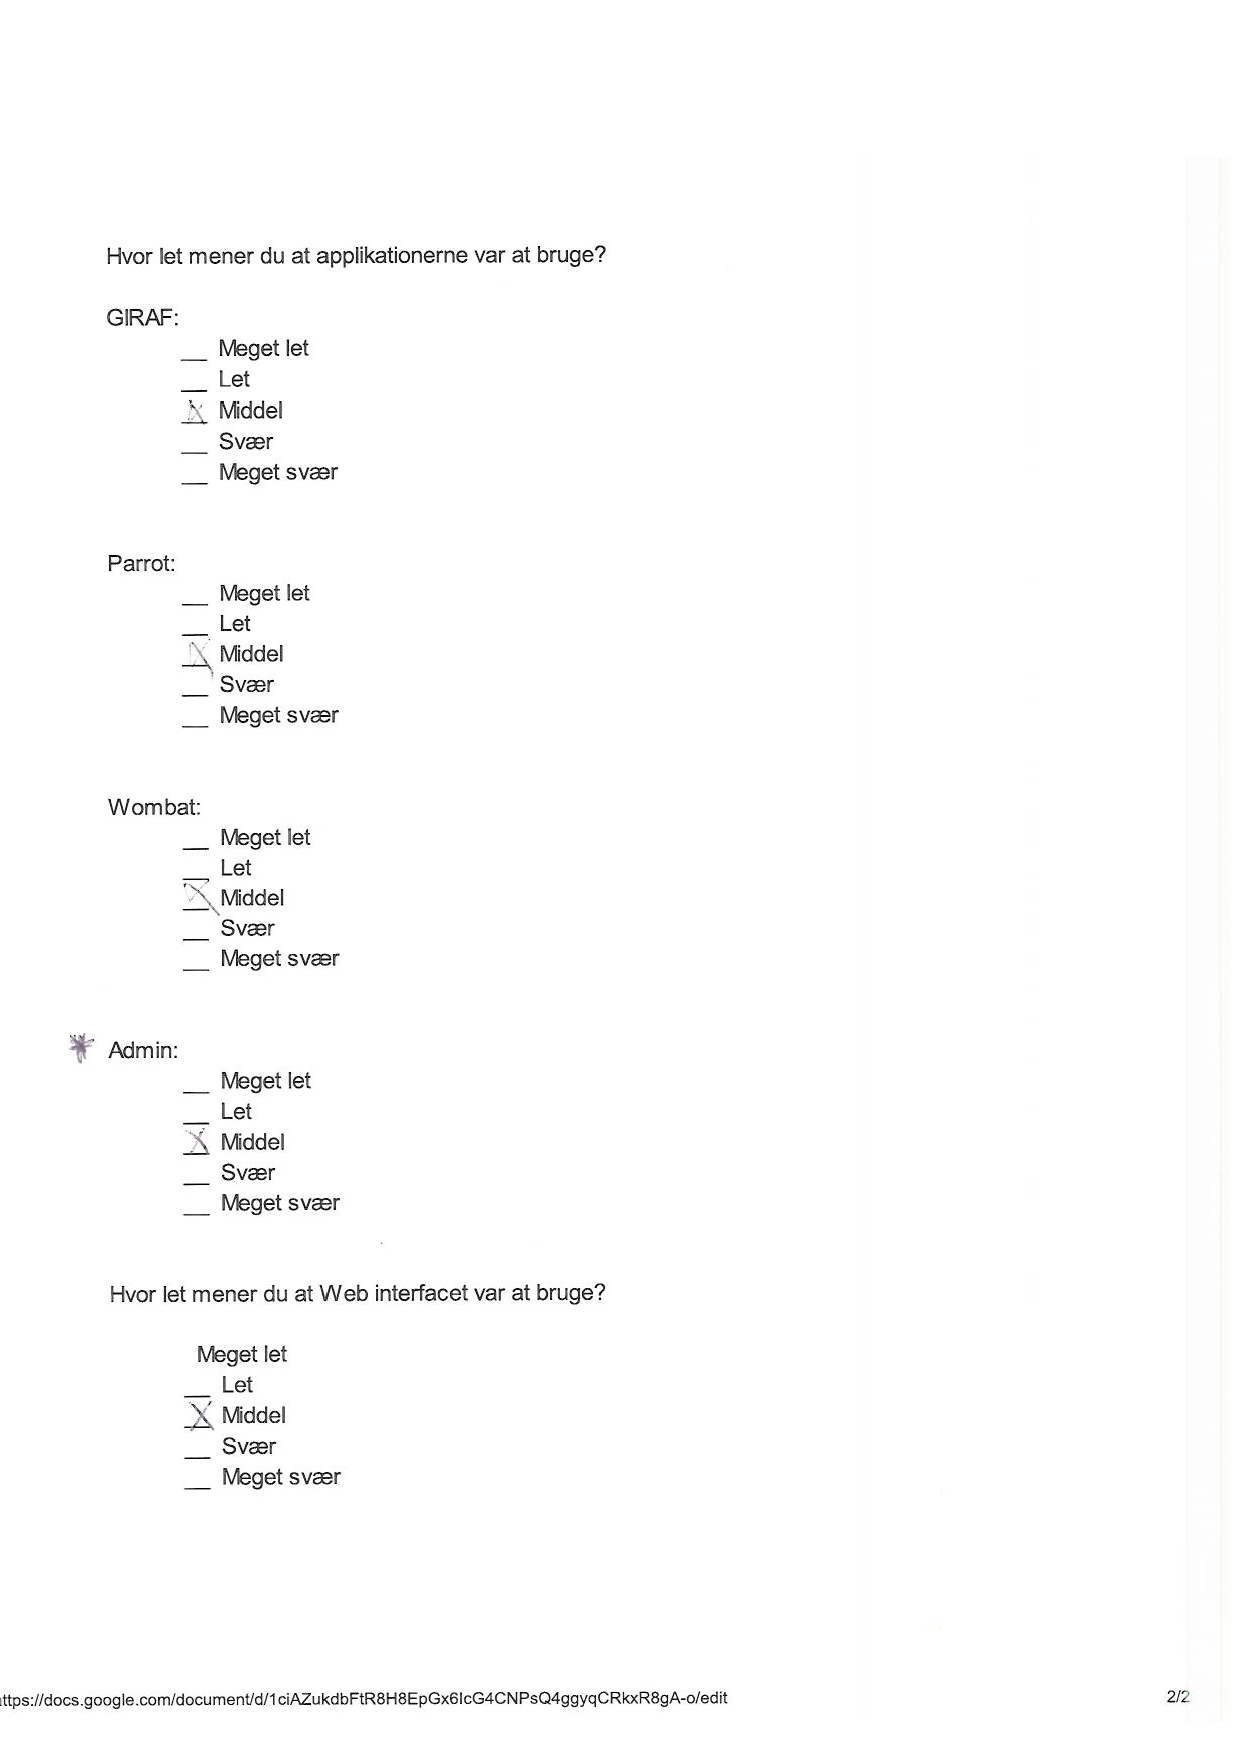
\includegraphics{Appendix/demo_m2.pdf}
	\label{fig:demo_t}
\end{figure}

\begin{figure}[h]
	\centering
		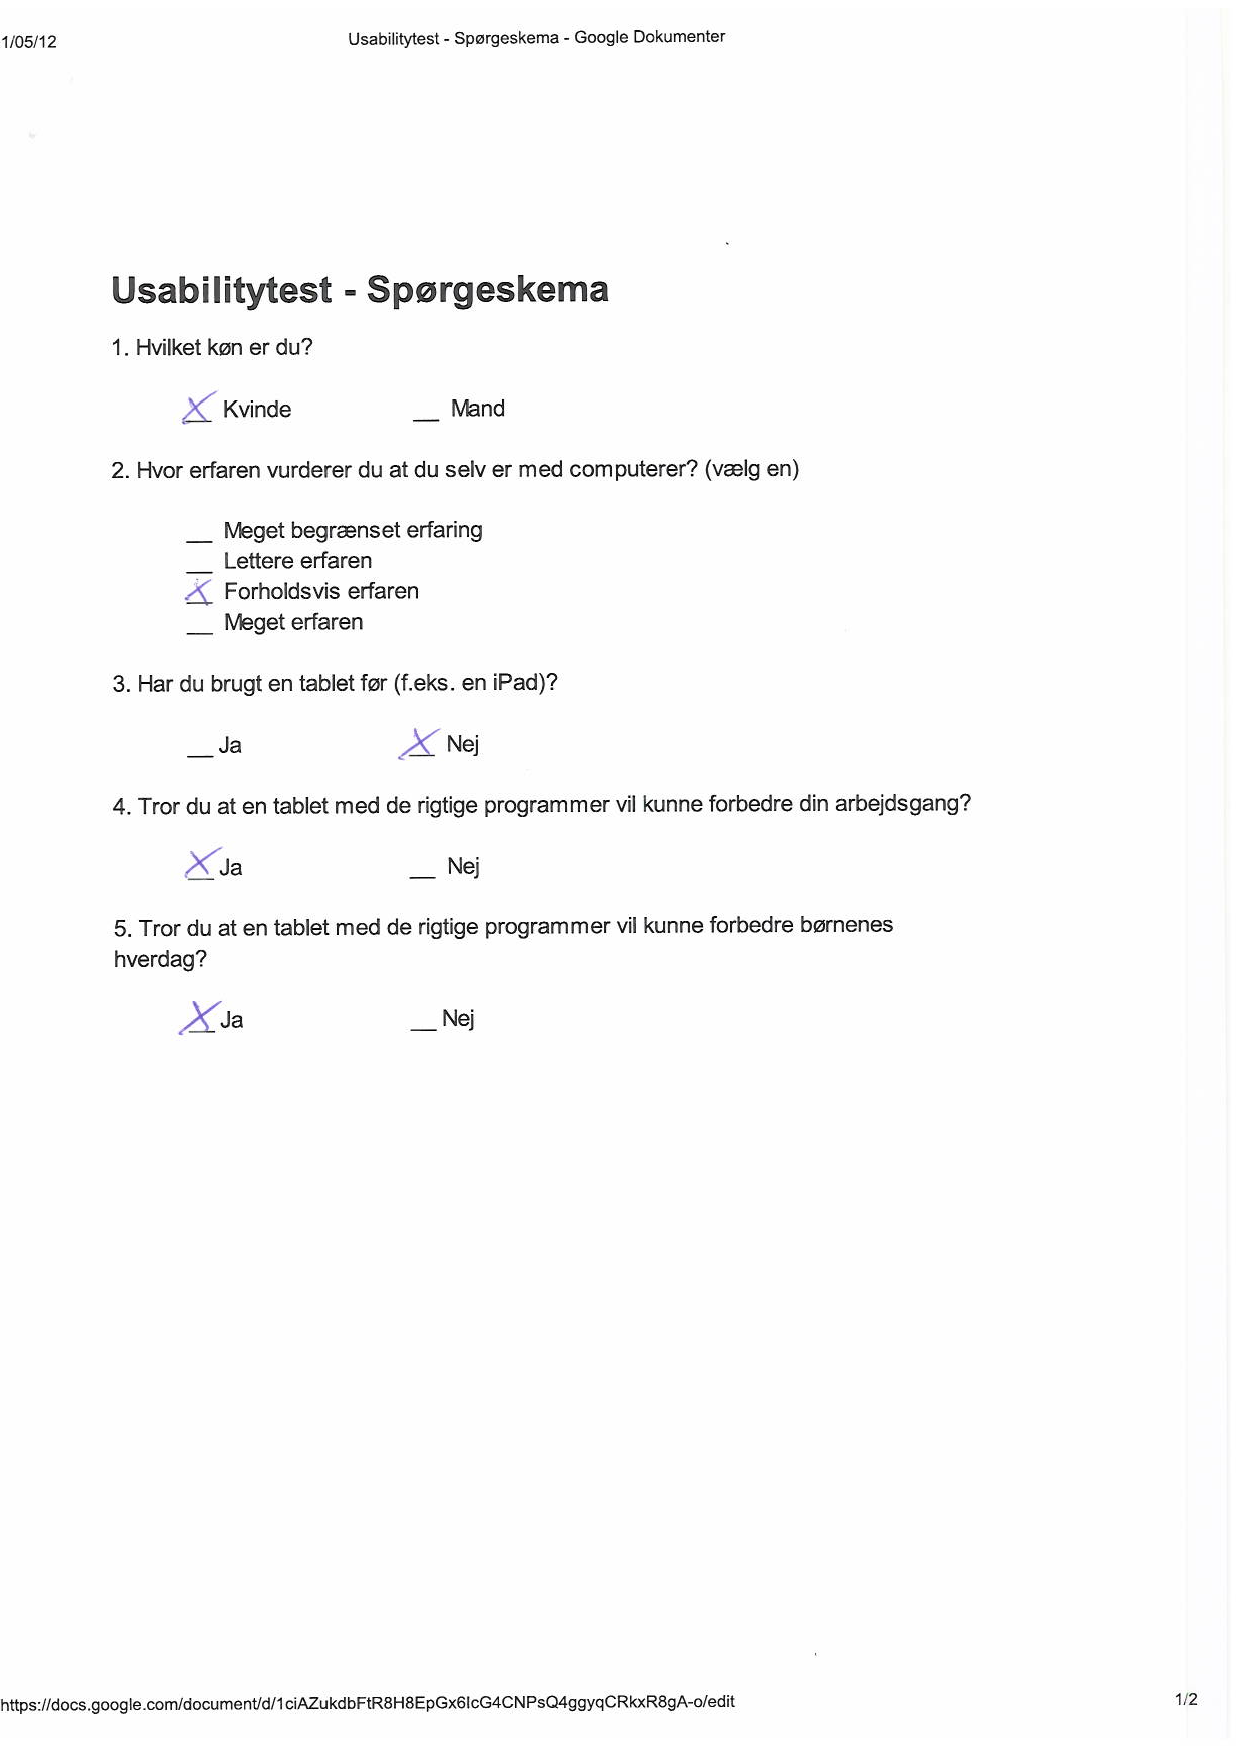
\includegraphics{Appendix/demo_t1.pdf}
	\label{fig:demo_t}
\end{figure}

\begin{figure}[h]
	\centering
		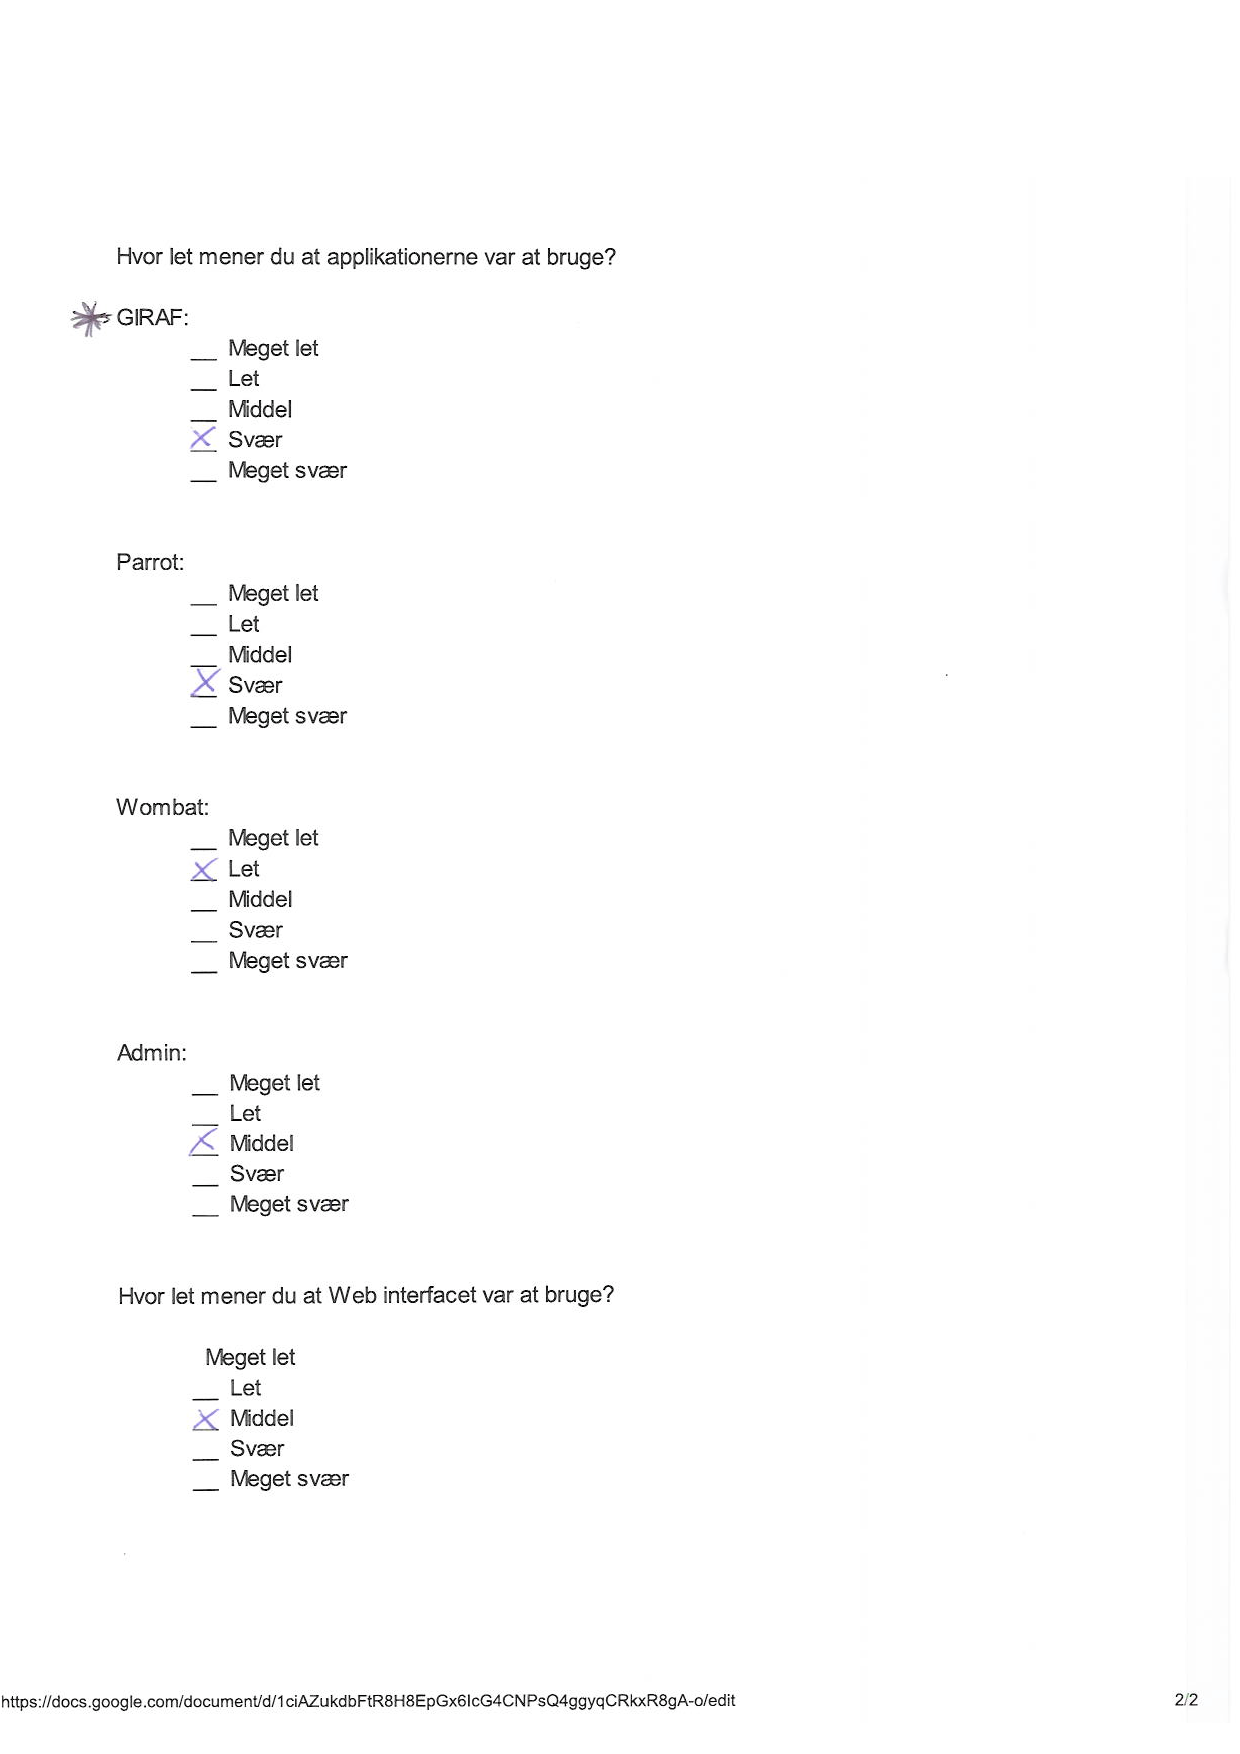
\includegraphics{Appendix/demo_t2.pdf}
	\label{fig:demo_t}
\end{figure}

\begin{figure}[h]
	\centering
		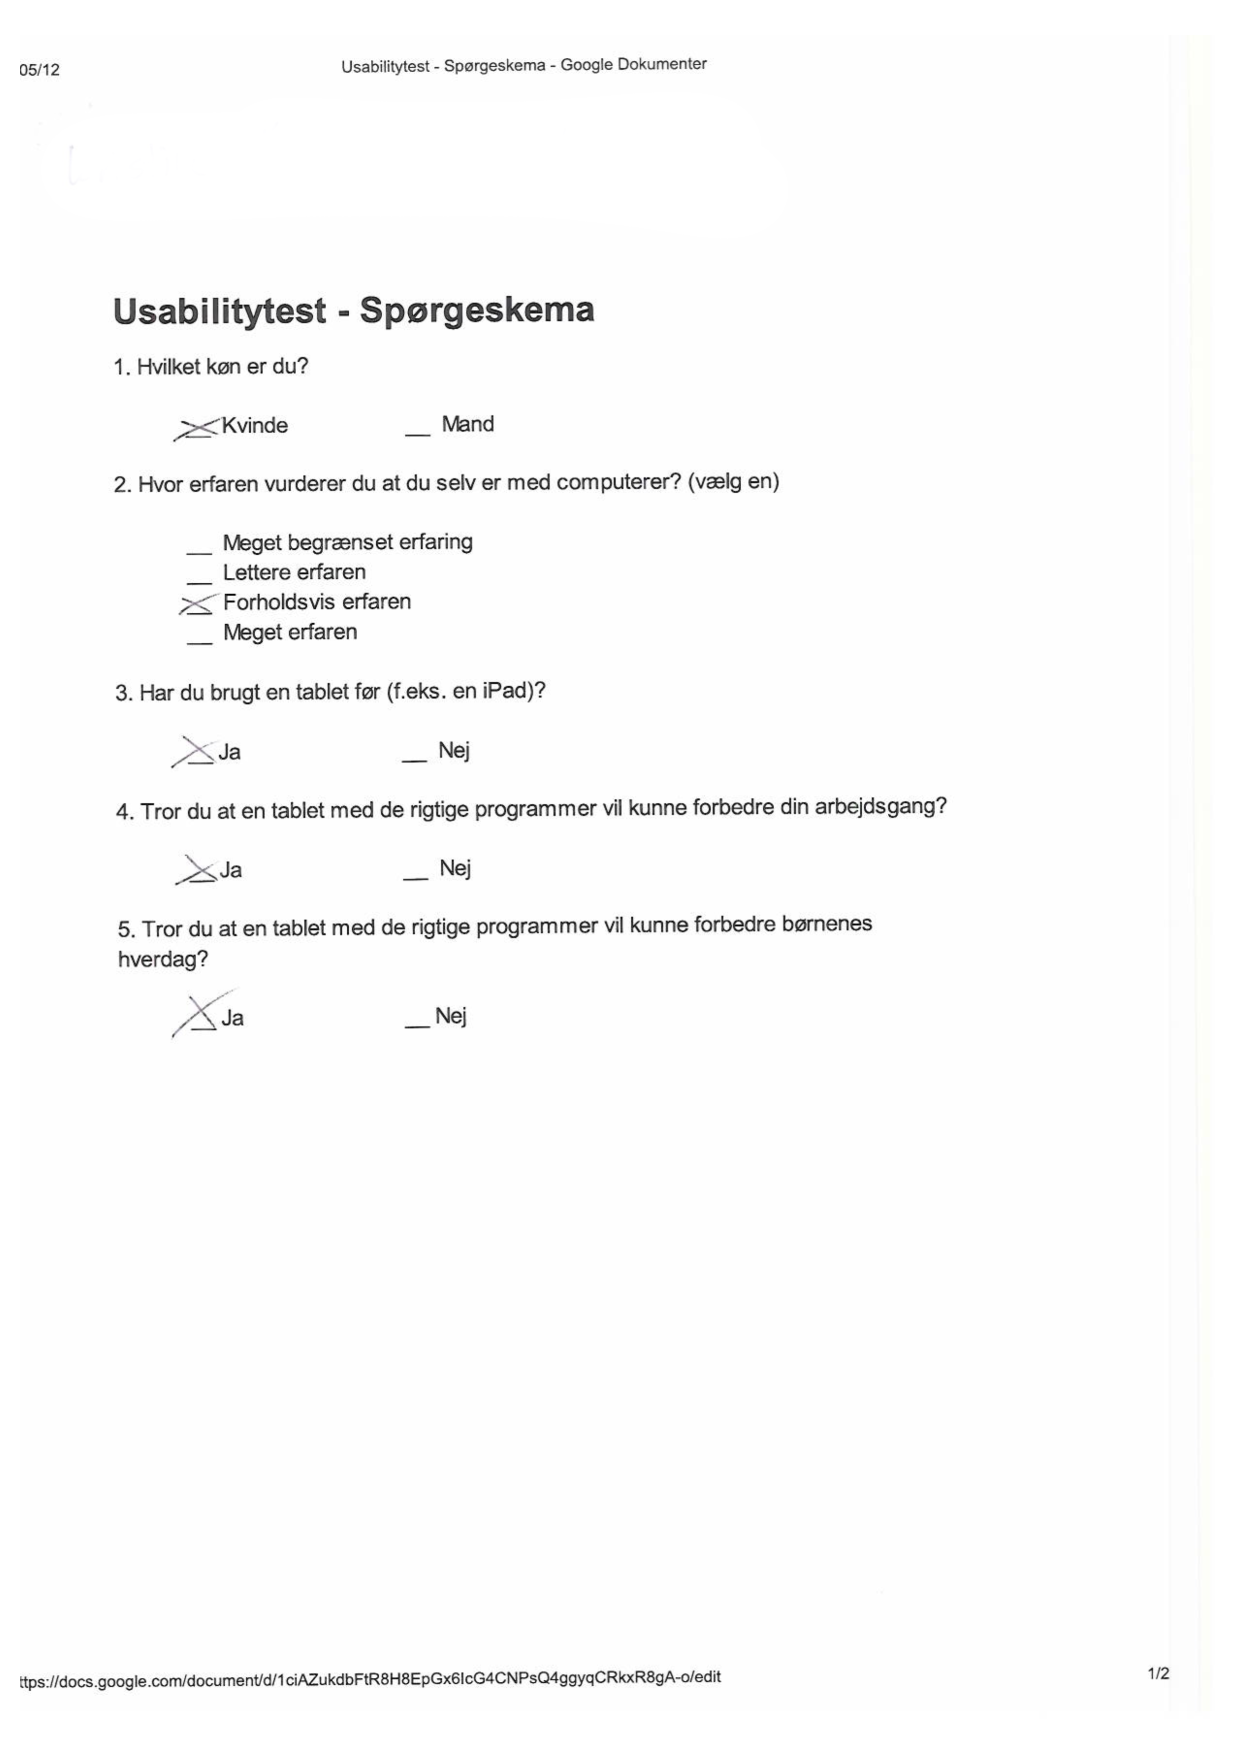
\includegraphics{Appendix/demo_k1.pdf}
	\label{fig:demo_t}
\end{figure}

\begin{figure}[h]
	\centering
		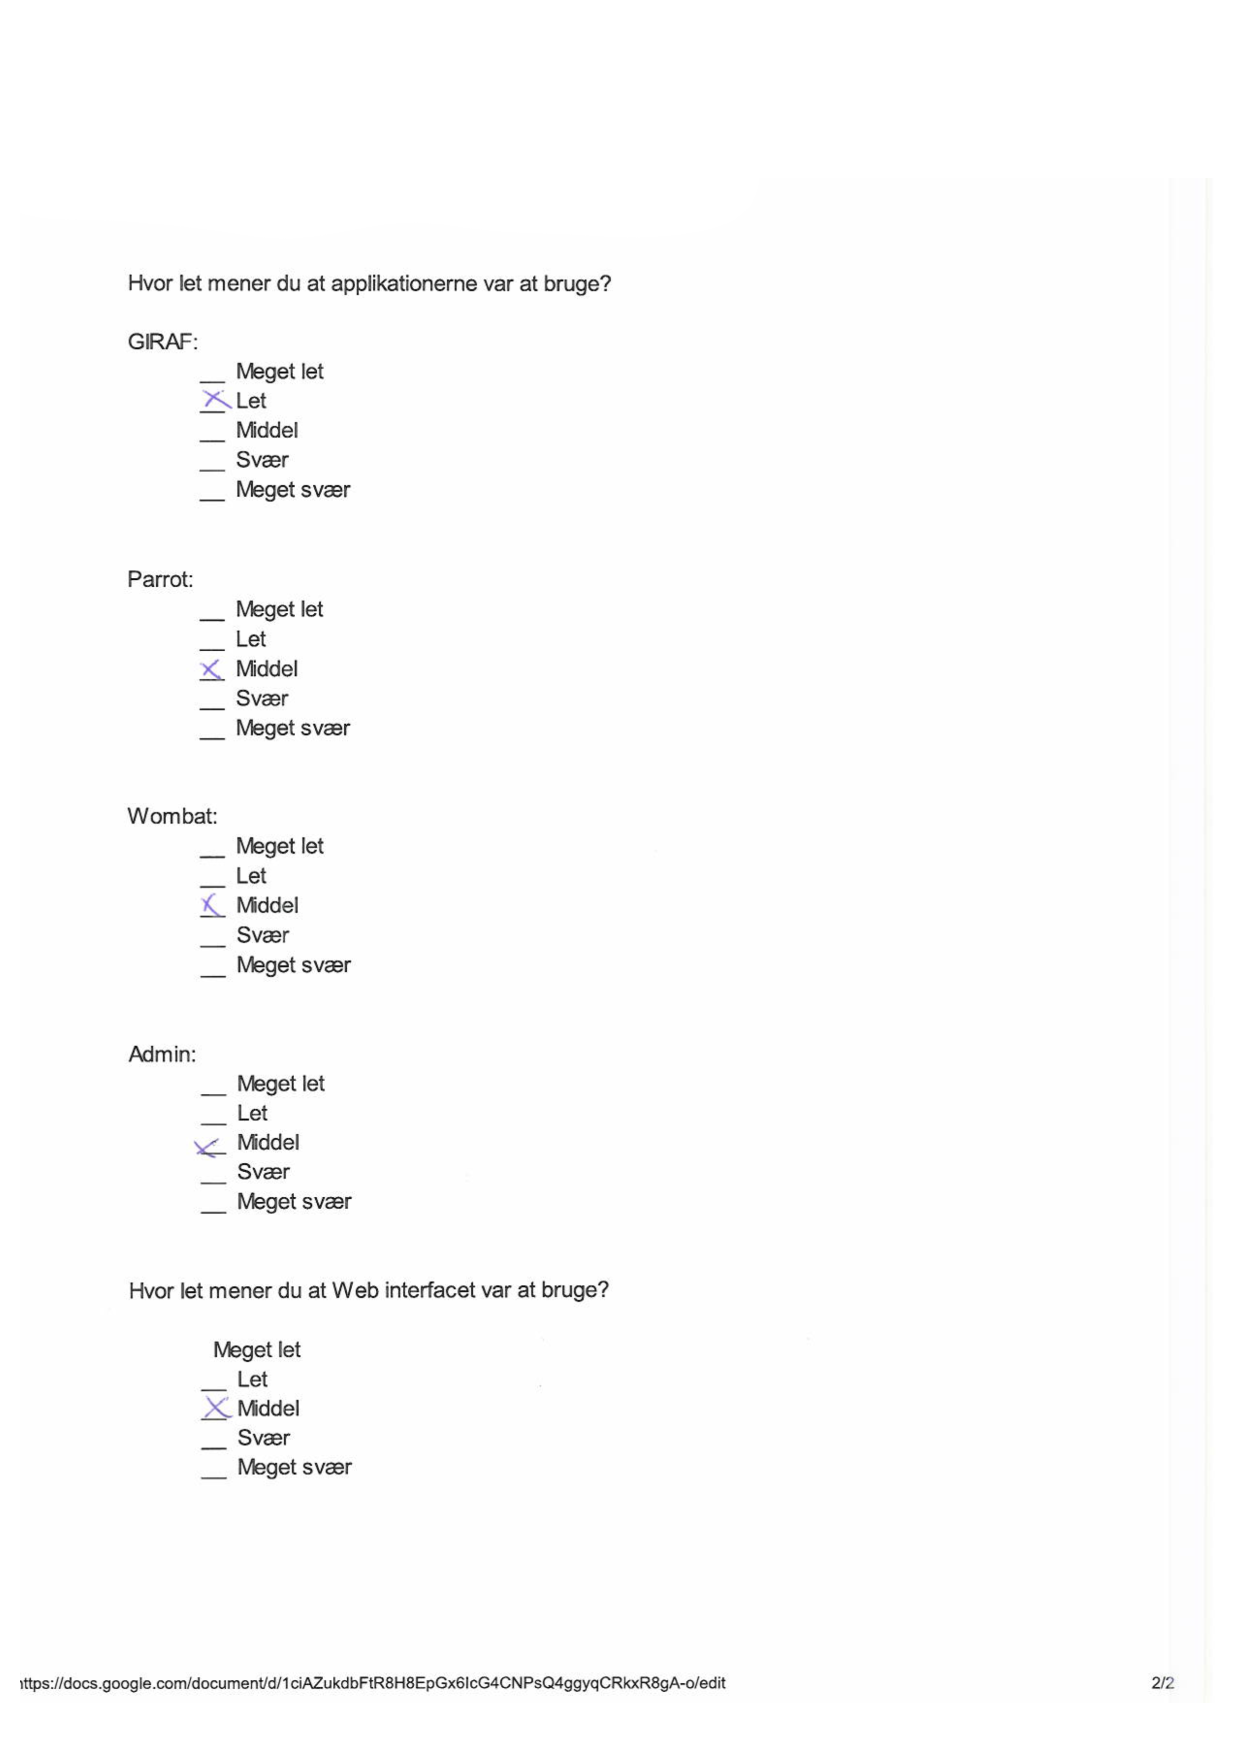
\includegraphics{Appendix/demo_k2.pdf}
	\label{fig:demo_t}
\end{figure}

\begin{figure}[h]
	\centering
		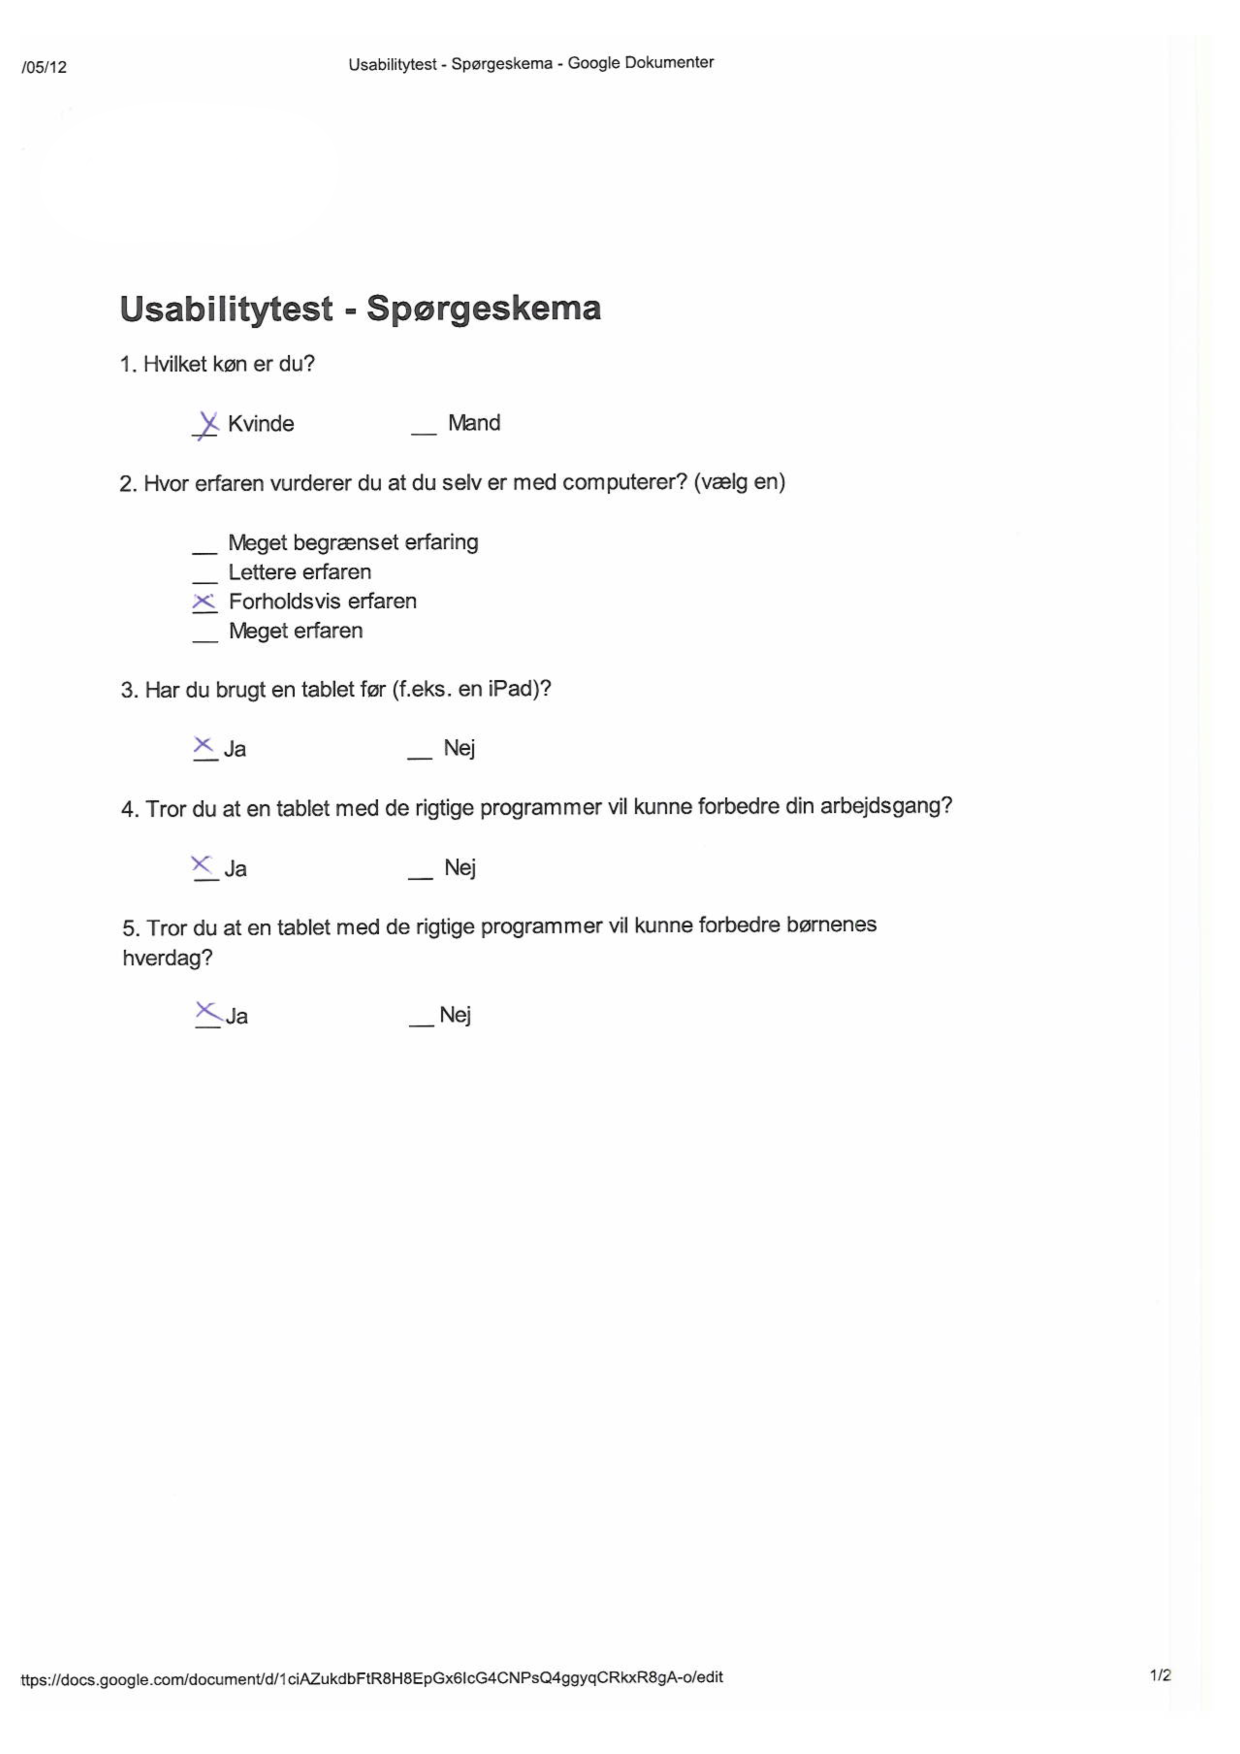
\includegraphics{Appendix/demo_ma1.pdf}
	\label{fig:demo_t}
\end{figure}

\begin{figure}[h]
	\centering
		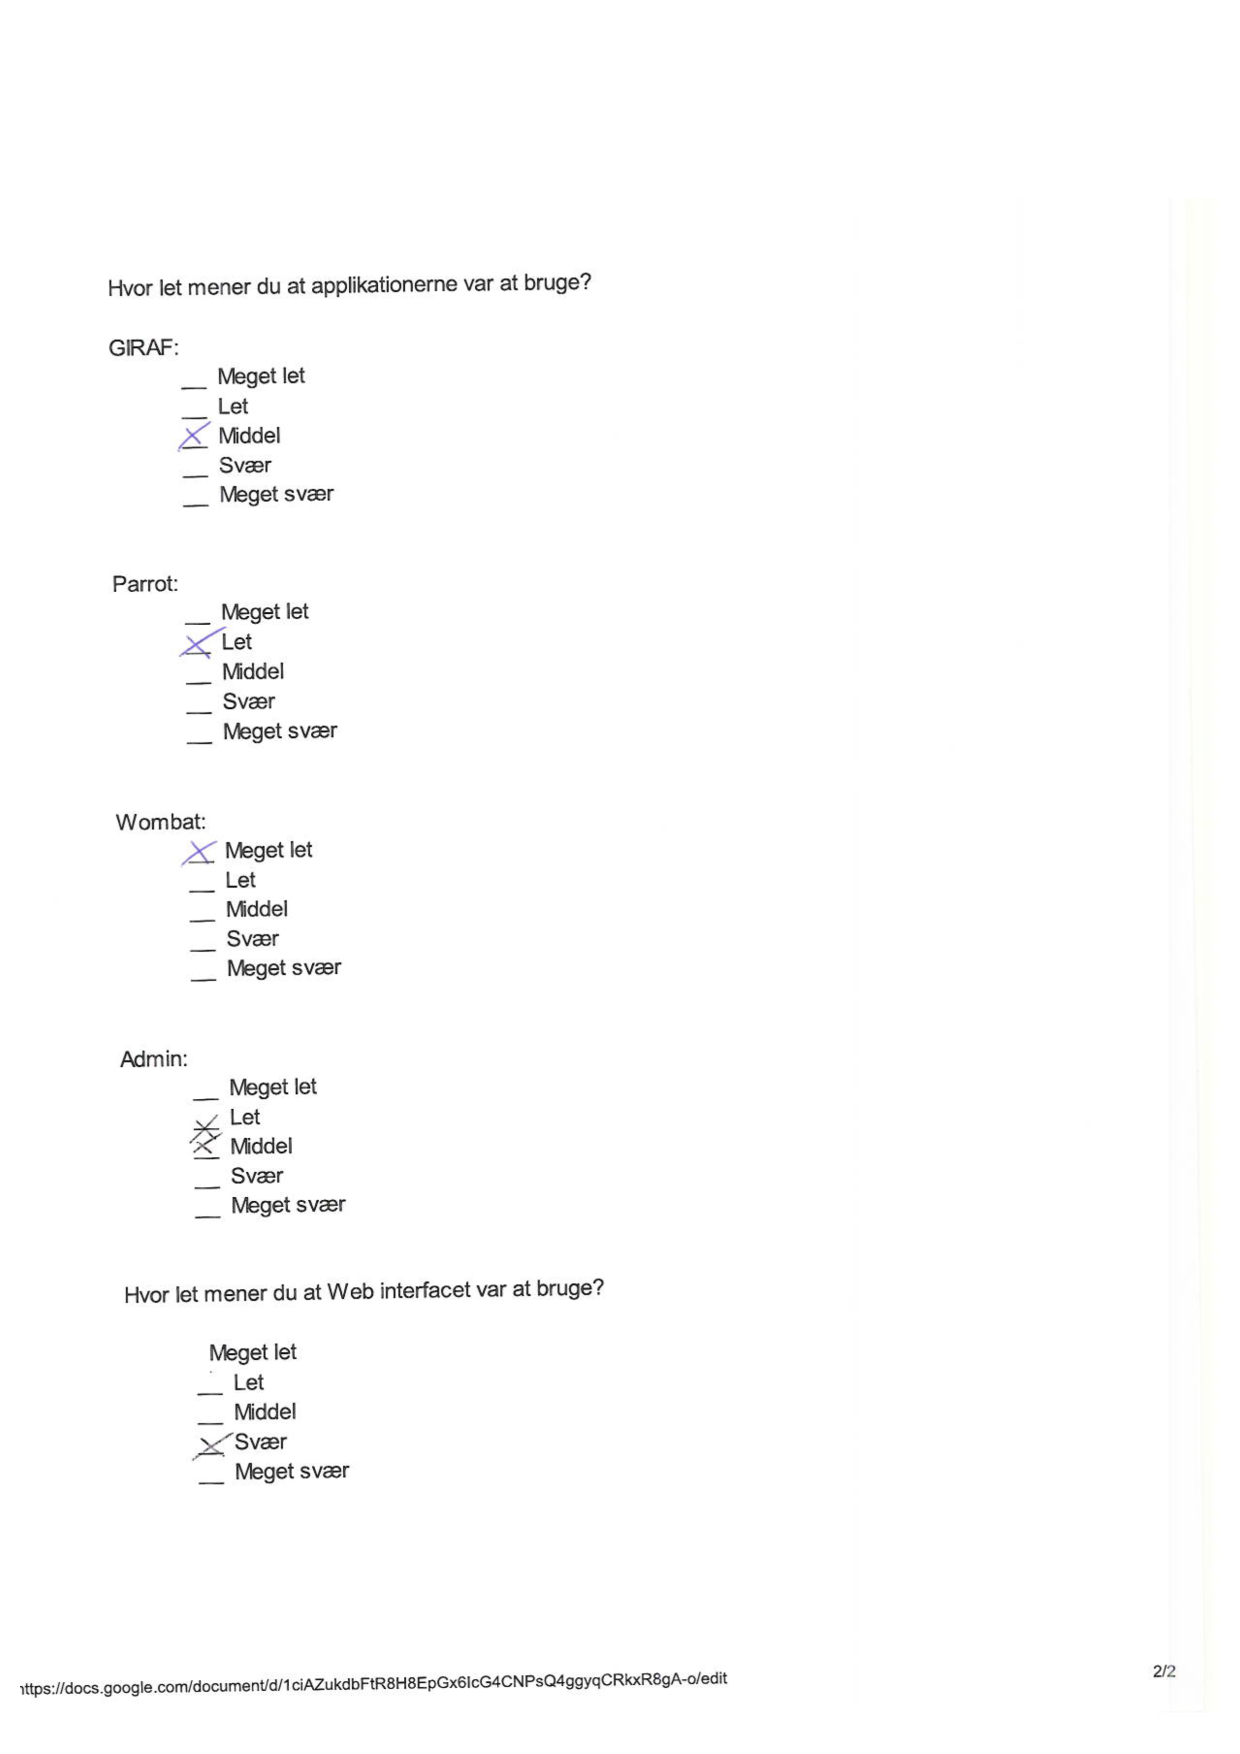
\includegraphics{Appendix/demo_ma2.pdf}
	\label{fig:demo_t}
\end{figure}

\section{Usability Assignments}
\label{sec:usabilityAss}
Admin applikation er en applikation der skal bruges til at styre informationer fra hver enkelt institution. Dette kan g\o{}re ved at manipulere data omkring institutioner og brugere.

Usability Opgaver:
\begin{itemize}
\item Opret en ny barne profil med f\o{}lgende informationer:
\begin{itemize}
		\item navn: 			Thomas Thomasen
	\item telefonnummer: 	12345678
		\item Afdeling:		Myretuen
		\end{itemize}
\item F\aa{} vist den nu oprettede barne profils informationer.
\item Find min profil og rediger navnet p\aa{} profilen fra Tony Stark til dit eget navn.
\item Tilf\o{}j den nu oprettede Thomas Thomasen til mine b\o{}rn.
\item Tilf\o{}j Applikationerne Wombat og Parrot til barnet Thomas Thomasen.
\item Fjern Thomas Thomasen fra afdelingen Myretuen.
\item Tilf\o{}j Thomas Thomasen til afdelingen Bikuben.
\end{itemize}

\section{Unit Test Results}
\label{app:unitTestResults}
In this section the results for the remaing unit tests can be found.

\begin{figure}[h]
	\centering
		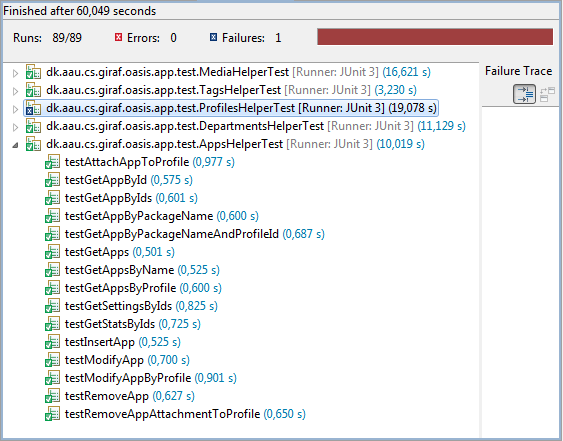
\includegraphics[width=\textwidth]{Images/unit_testing/app_helper_tests.PNG}
	\caption{The result from the \texttt{appsHelper} tests.}
	\label{fig:app_helper_tests}
\end{figure}

\begin{figure}[h]
	\centering
		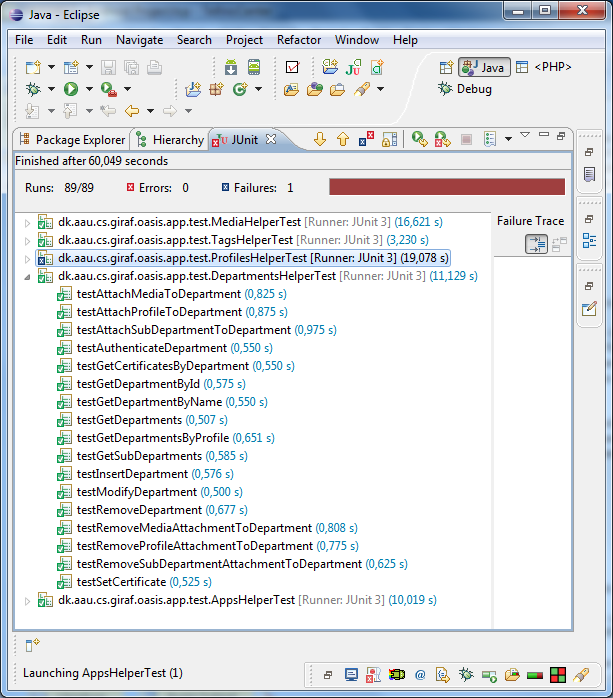
\includegraphics[width=\textwidth]{Images/unit_testing/department_helper_tests.PNG}
	\caption{The result from the \texttt{departmentHelper} tests.}
	\label{fig:department_helper_tests}
\end{figure}

\begin{figure}[h]
	\centering
		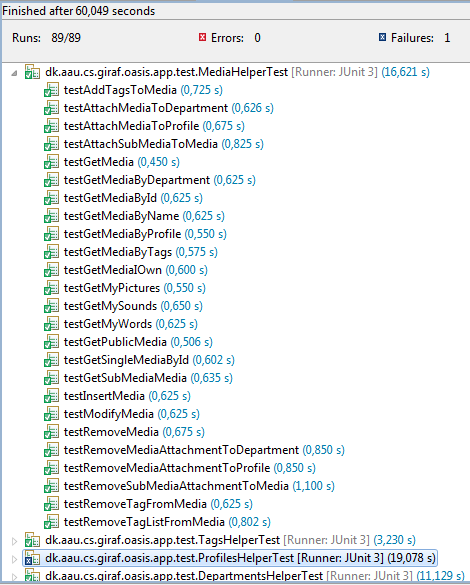
\includegraphics[width=\textwidth]{Images/unit_testing/media_helper_tests.PNG}
	\caption{The result from the \texttt{mediaHelper} tests.}
	\label{fig:media_helper_tests}
\end{figure}

\begin{figure}[h]
	\centering
		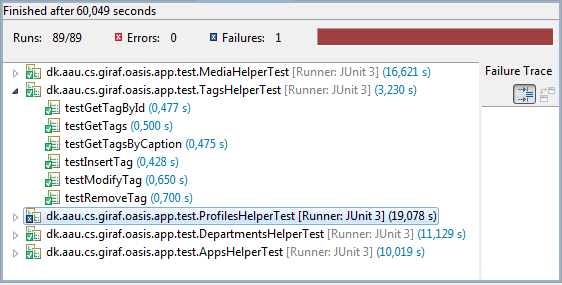
\includegraphics[width=\textwidth]{Images/unit_testing/tag_helper_tests.PNG}
	\caption{The result from the \texttt{tagsHelper} tests.}
	\label{fig:tag_helper_tests}
\end{figure}